% Copyright 2019 Clara Eleonore Pavillet

% Author: Clara Eleonore Pavillet
% Description: This is an unofficial Oxford University Beamer Template I made from scratch. Feel free to use it, modify it, share it.
% Version: 1.0

\documentclass{beamer}
\usepackage{animate}
\newcommand{\comment}[1]{}

% Load Packages
\usepackage[utf8]{inputenc}
\usepackage{xcolor}
\usepackage{tikz}
\usetikzlibrary{positioning,calc}
\usepackage{graphicx}
\usepackage{hyperref}
\usepackage{amsmath}
\usepackage{listings}
%\usepackage{fontawesome}

% Define Commands
\newcommand*{\ClipSep}{0.06cm} %To adjust footer logo
\newcommand{\E}{\mathrm{e}\,} %\def\I{e} % used to defined e for exp(x), see later what it should be
\newcommand{\ud}{\mathrm{d}}
\lstset{numbers=left, numberstyle=\tiny, stepnumber=1,firstnumber=1,breaklines=true,
    numbersep=5pt,language=Python,
    stringstyle=\ttfamily,
    basicstyle=\footnotesize, 
    showstringspaces=false
}

\usetheme{oxonian}

\title{LXe scintillation model}
\begin{document}

{\setbeamertemplate{footline}{} 
\frame{\titlepage}}

\begin{frame}{Objective}
We want to use the data collected by the Cs and Co runs to estimate the parameters for the scintillation model.\\
In the following we show that there is a $\delta(t)$ component in the model with high statistical significance and propose how to go on to claim a discovery. 
\end{frame}


\begin{frame}{Signal Reconstruction}
%	\begin{center}
%	\animategraphics[loop,controls,width=0.6\linewidth]{10}{recon-}{0}{41}	
%	\end{center}
  
To study the temporal structure of the photon emission a processing algorithm uses a template of the average SPE signal to reconstruct the temporal PE pattern in each event for each PMT separately. The output of this process is the number of PEs created in the PMT in each digitization point.

\begin{figure}[h]
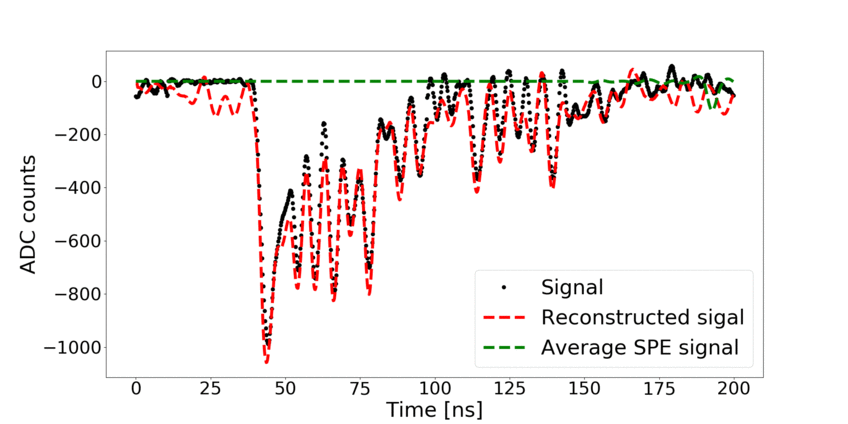
\includegraphics[width=0.5\linewidth]{recon-41.png}
\end{figure}

\begin{figure}[h]
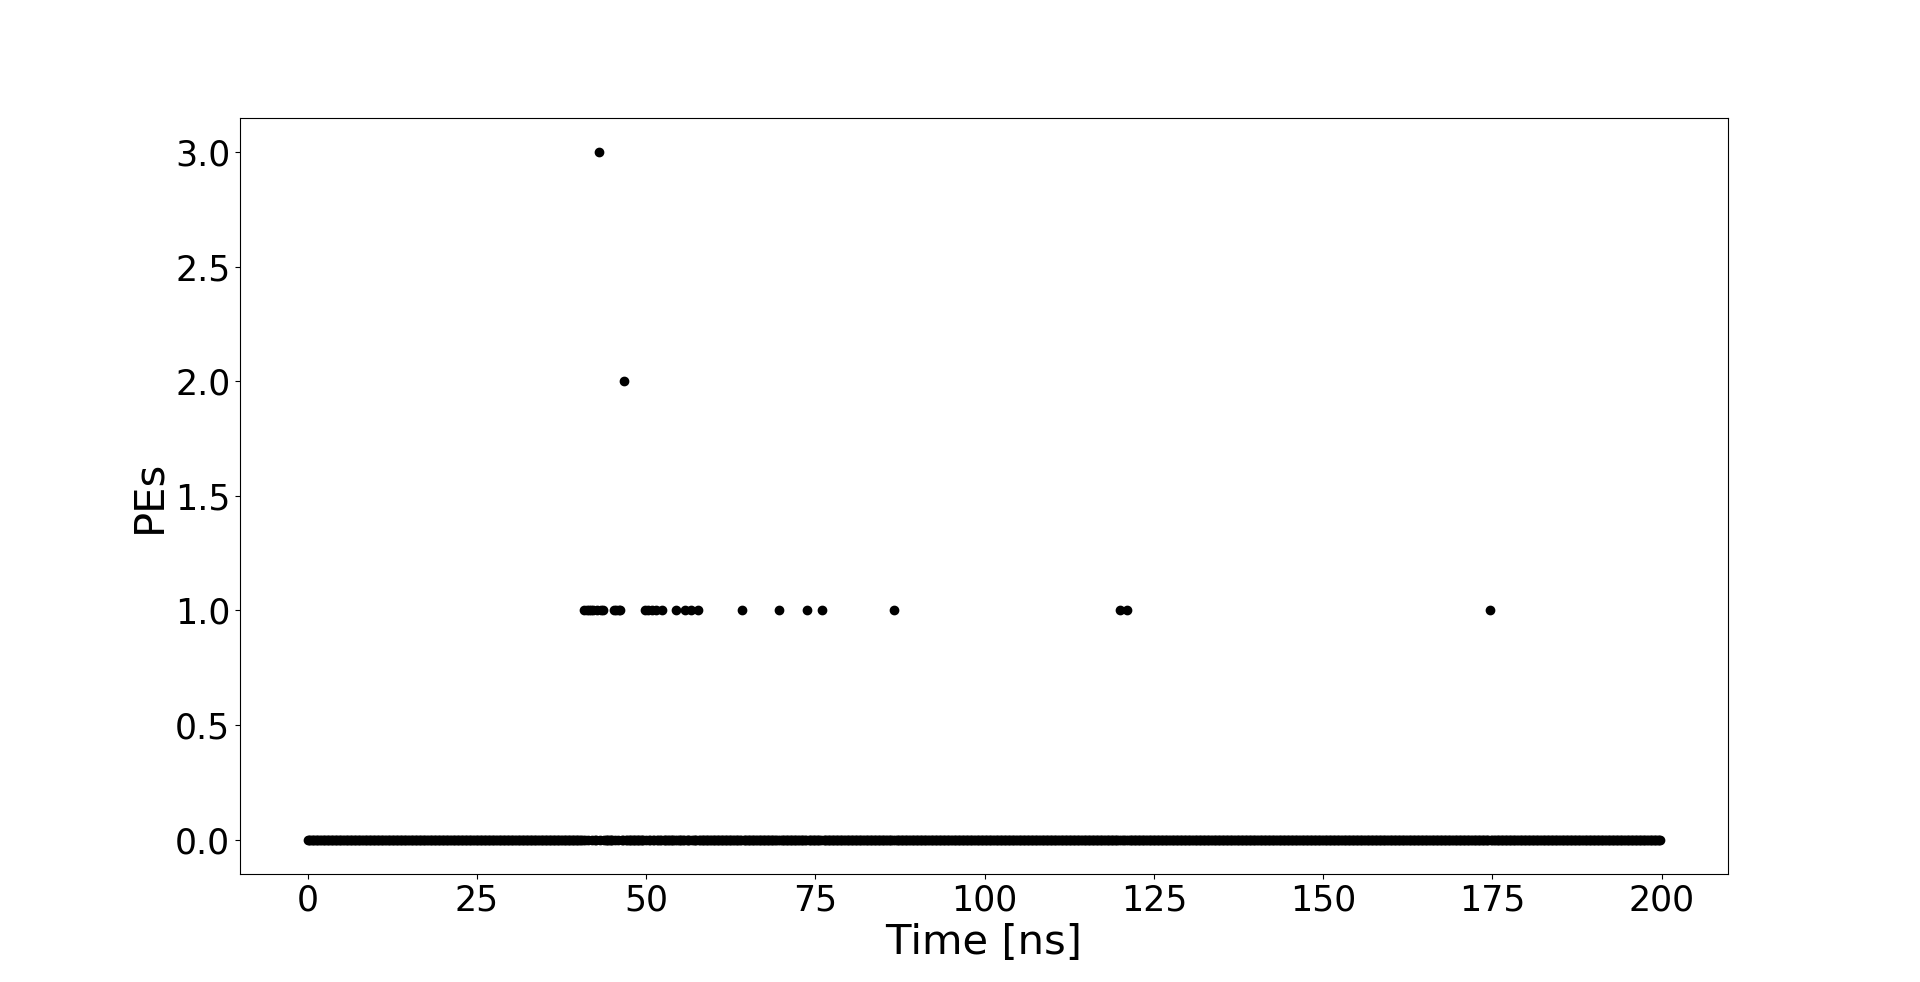
\includegraphics[width=0.5\linewidth]{PEs.png}
\end{figure}
\end{frame}

\begin{frame}{Reconstruction results}
\begin{figure}[h]
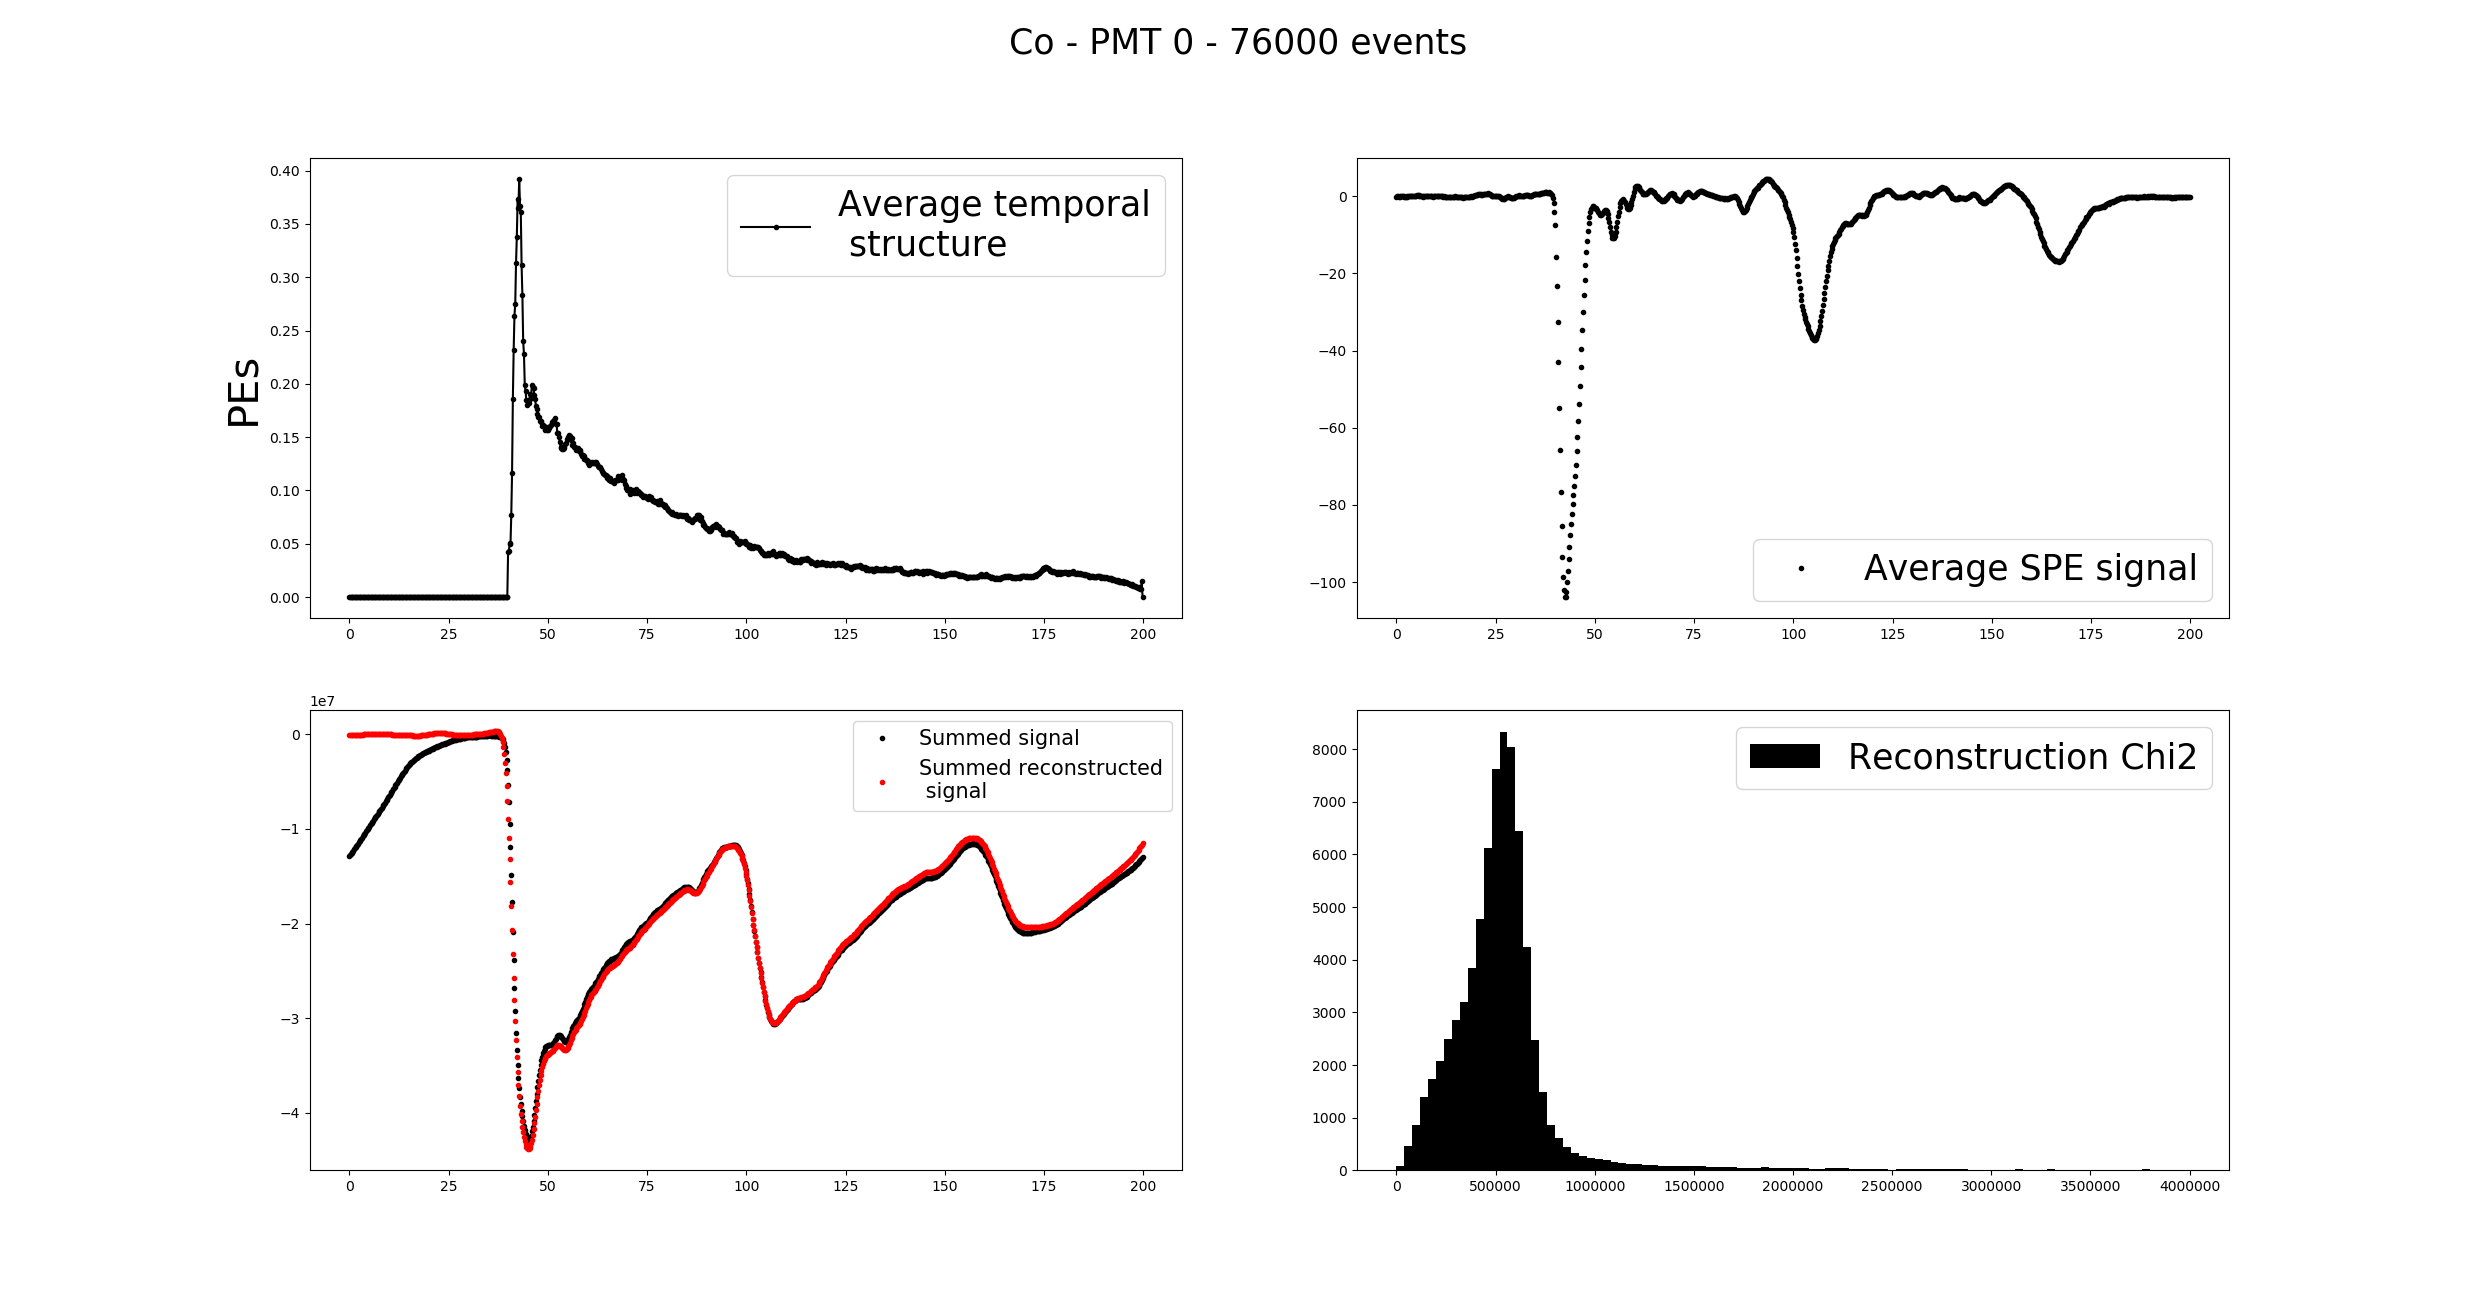
\includegraphics[width=1\linewidth]{resultCo0.png}
\end{figure}
\end{frame}


\begin{frame}{Reconstruction results}
\begin{figure}[h]
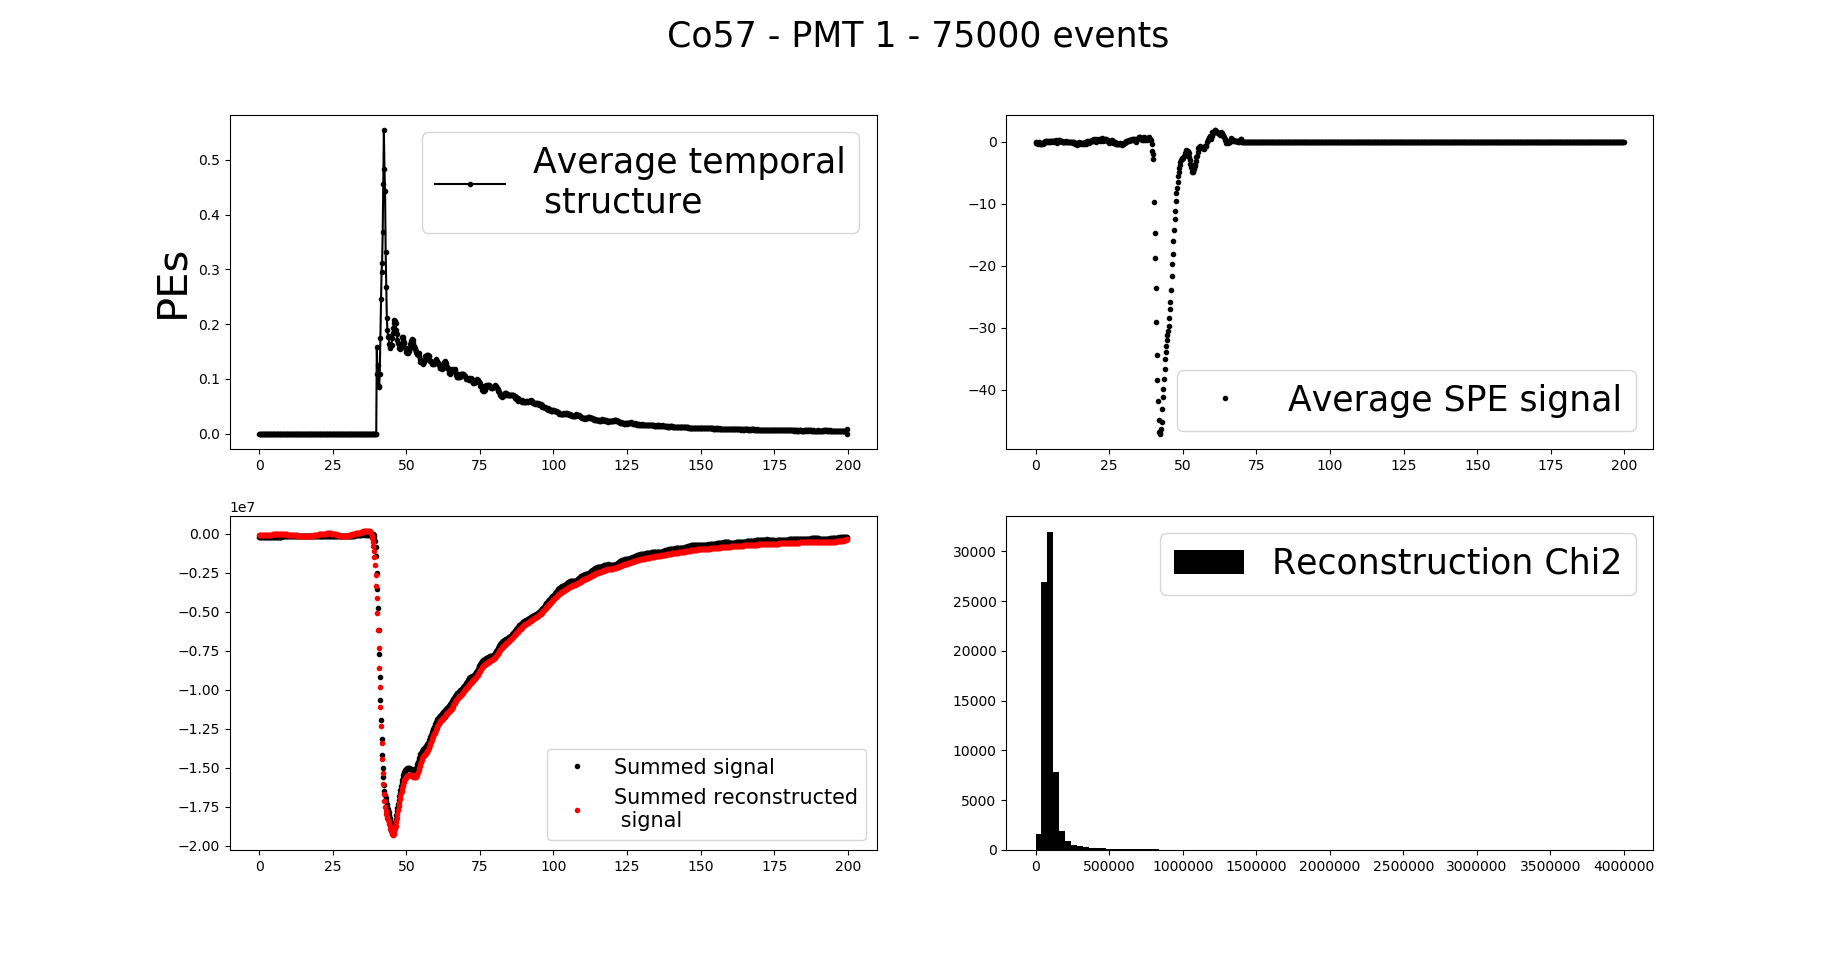
\includegraphics[width=1\linewidth]{resultCo1.png}
\end{figure}
\end{frame}

\begin{frame}{Reconstruction results}
\begin{figure}[h]
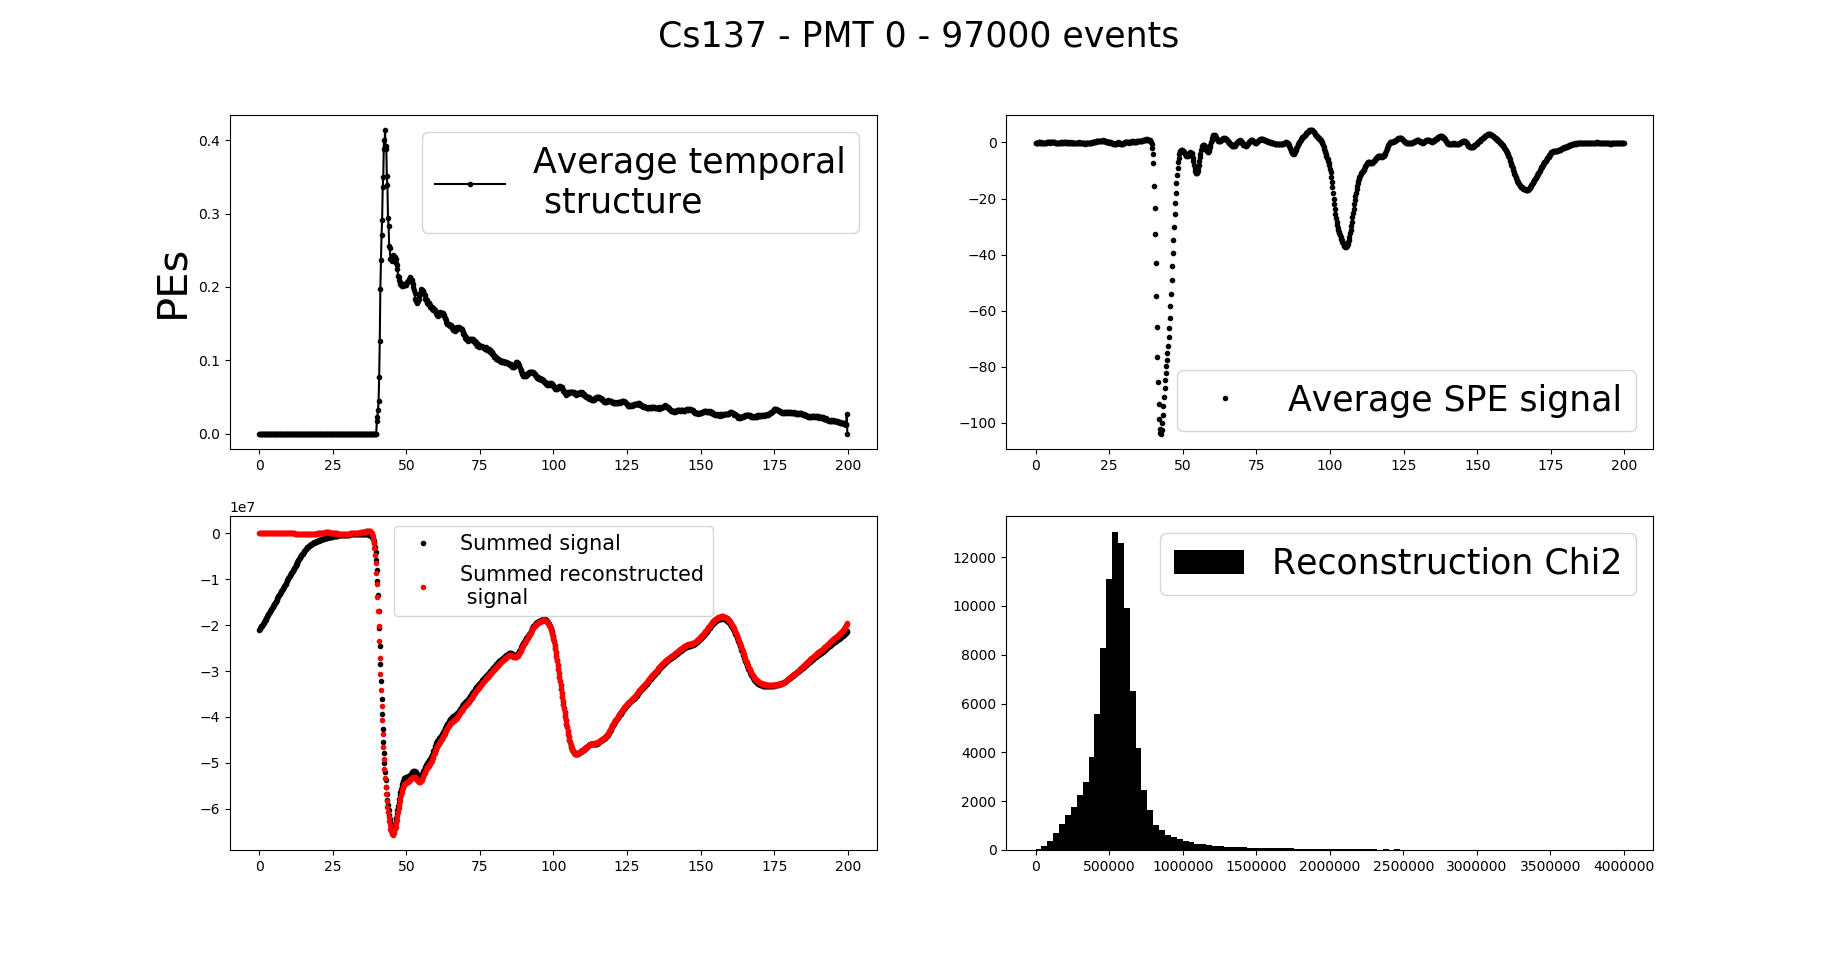
\includegraphics[width=1\linewidth]{resultCs0.png}
\end{figure}
\end{frame}

\begin{frame}
\begin{figure}[h]
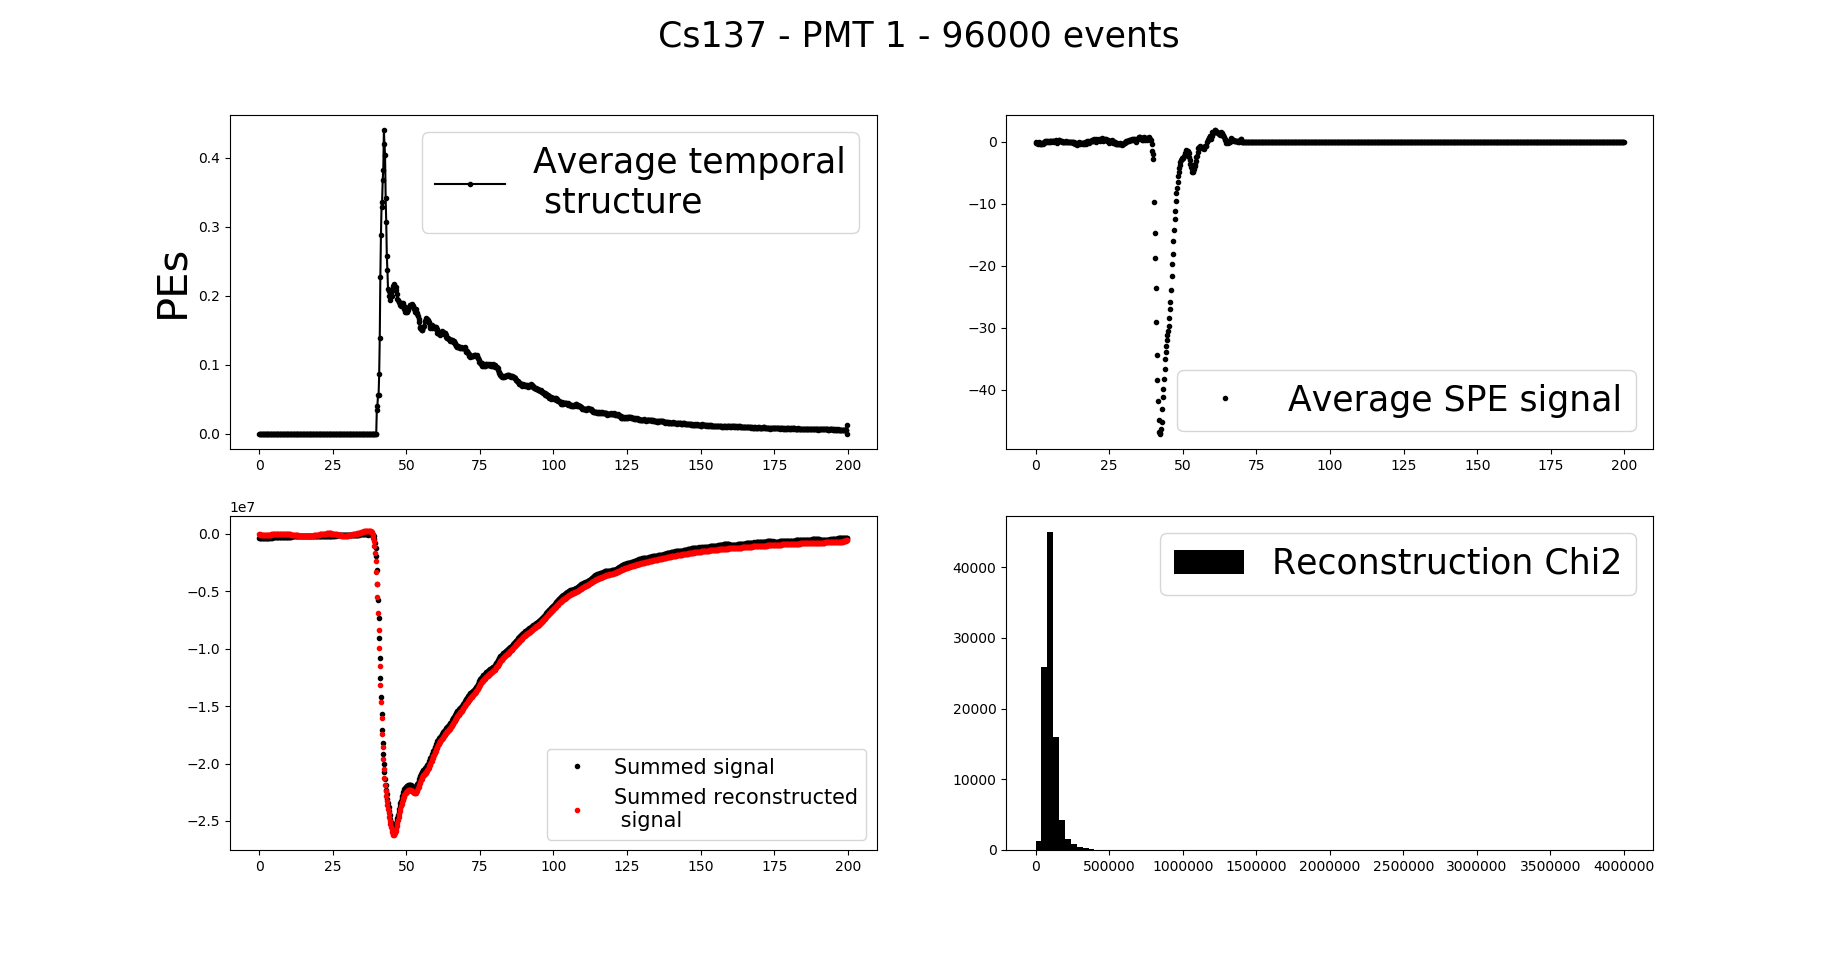
\includegraphics[width=1\linewidth]{resultCs1.png}
\end{figure}
\end{frame}

\begin{frame}
\begin{figure}[h]
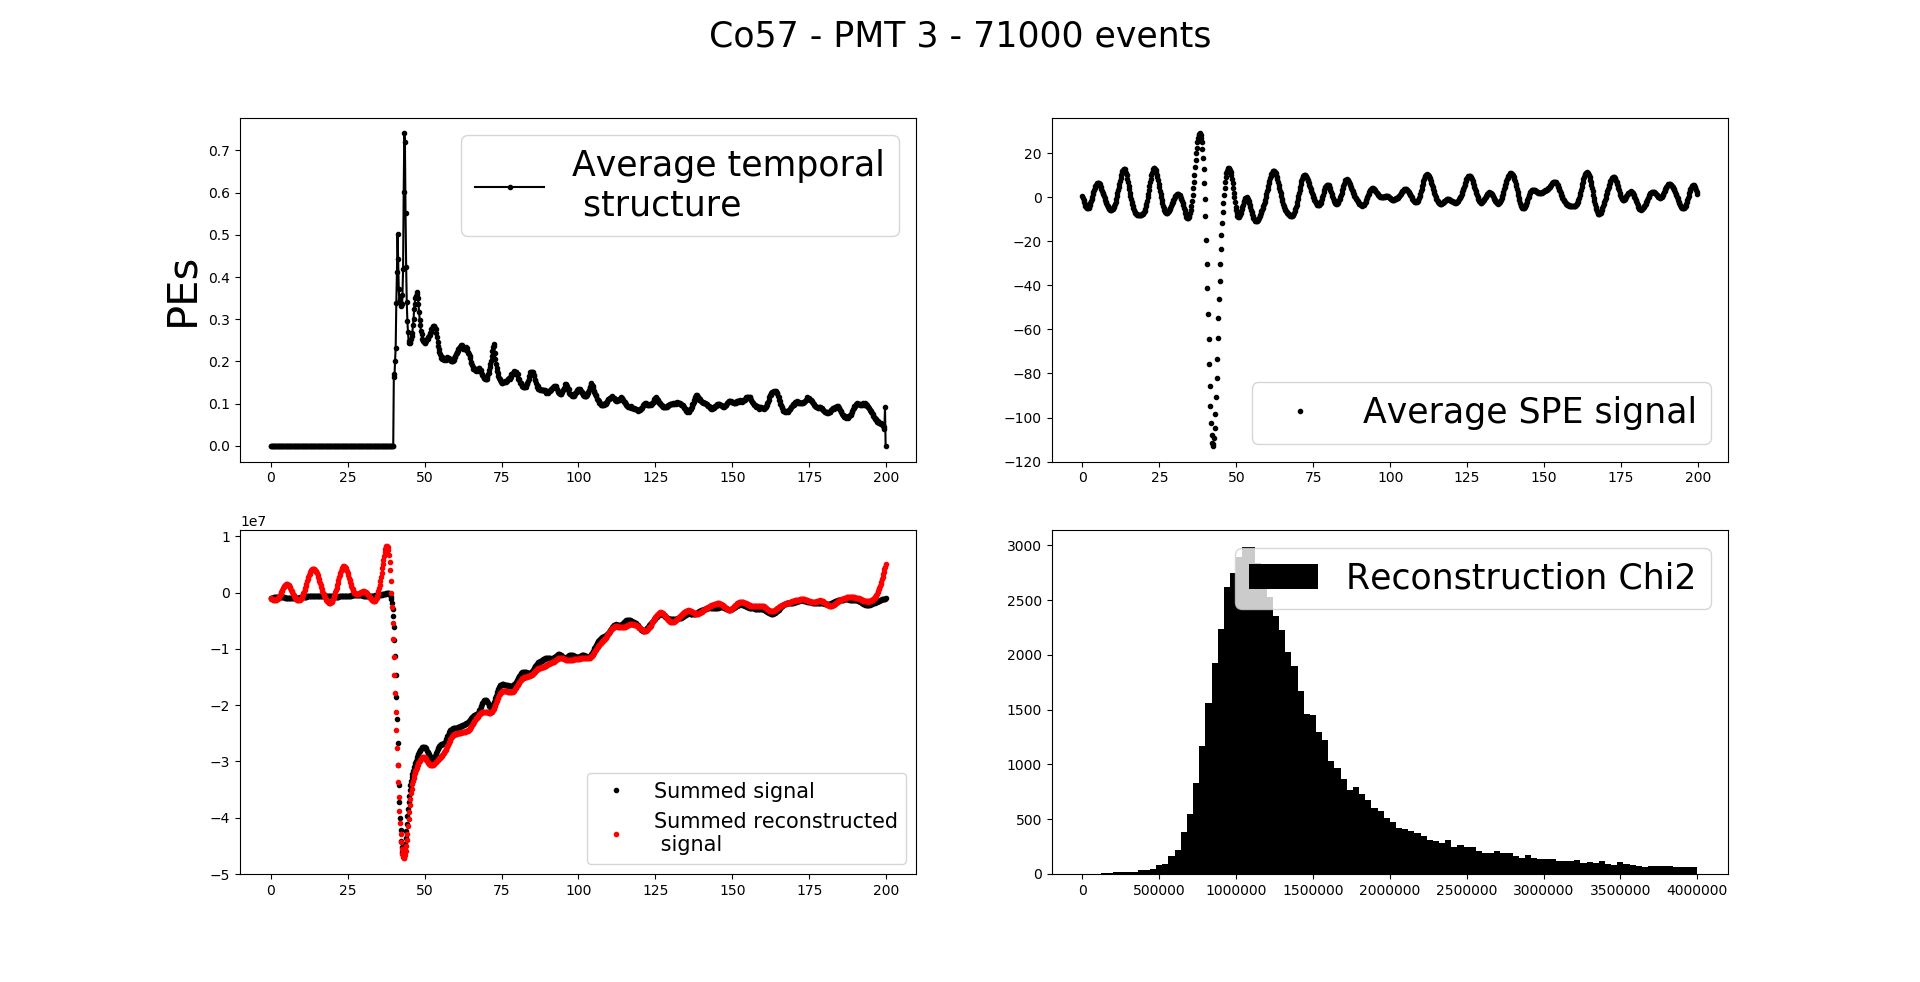
\includegraphics[width=1\linewidth]{resultCo3.png}
\end{figure}
\end{frame}

\begin{frame}
\begin{figure}[h]
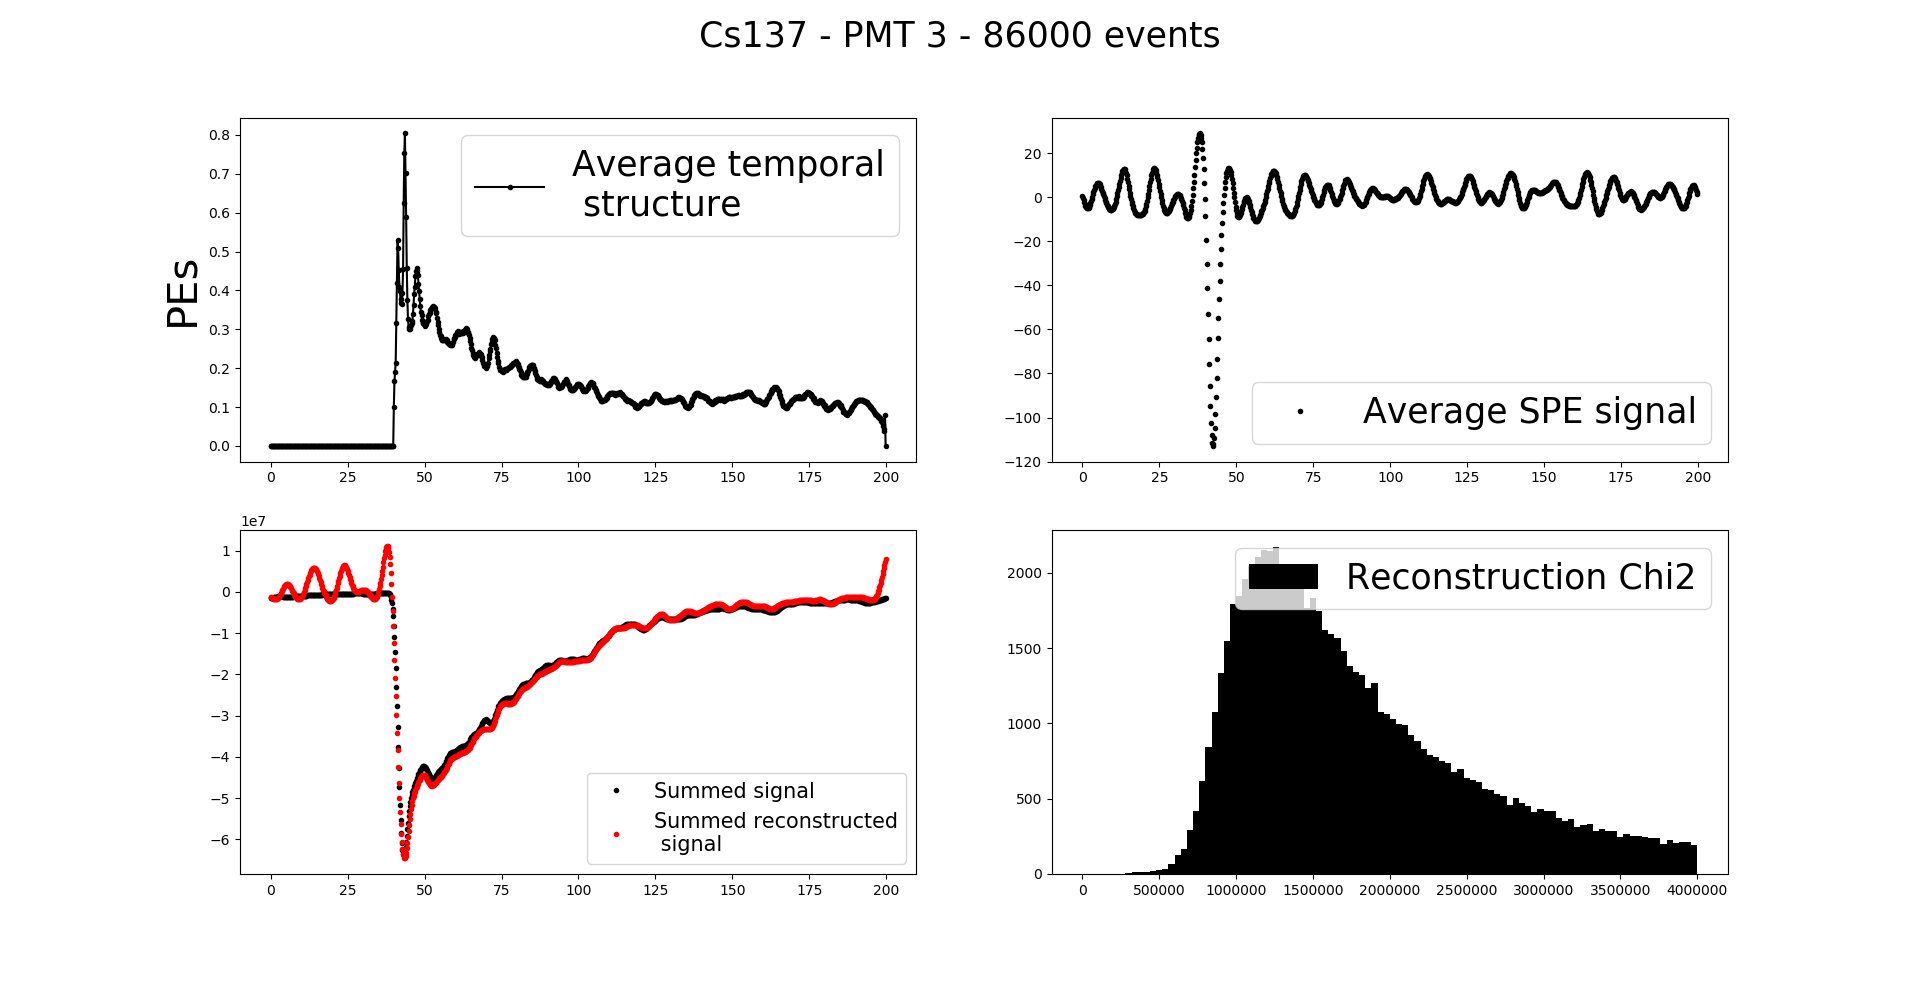
\includegraphics[width=1\linewidth]{resultCs3.png}
\end{figure}
\end{frame}

\begin{frame}{1 PMT Spectrum}
\begin{figure}[h]
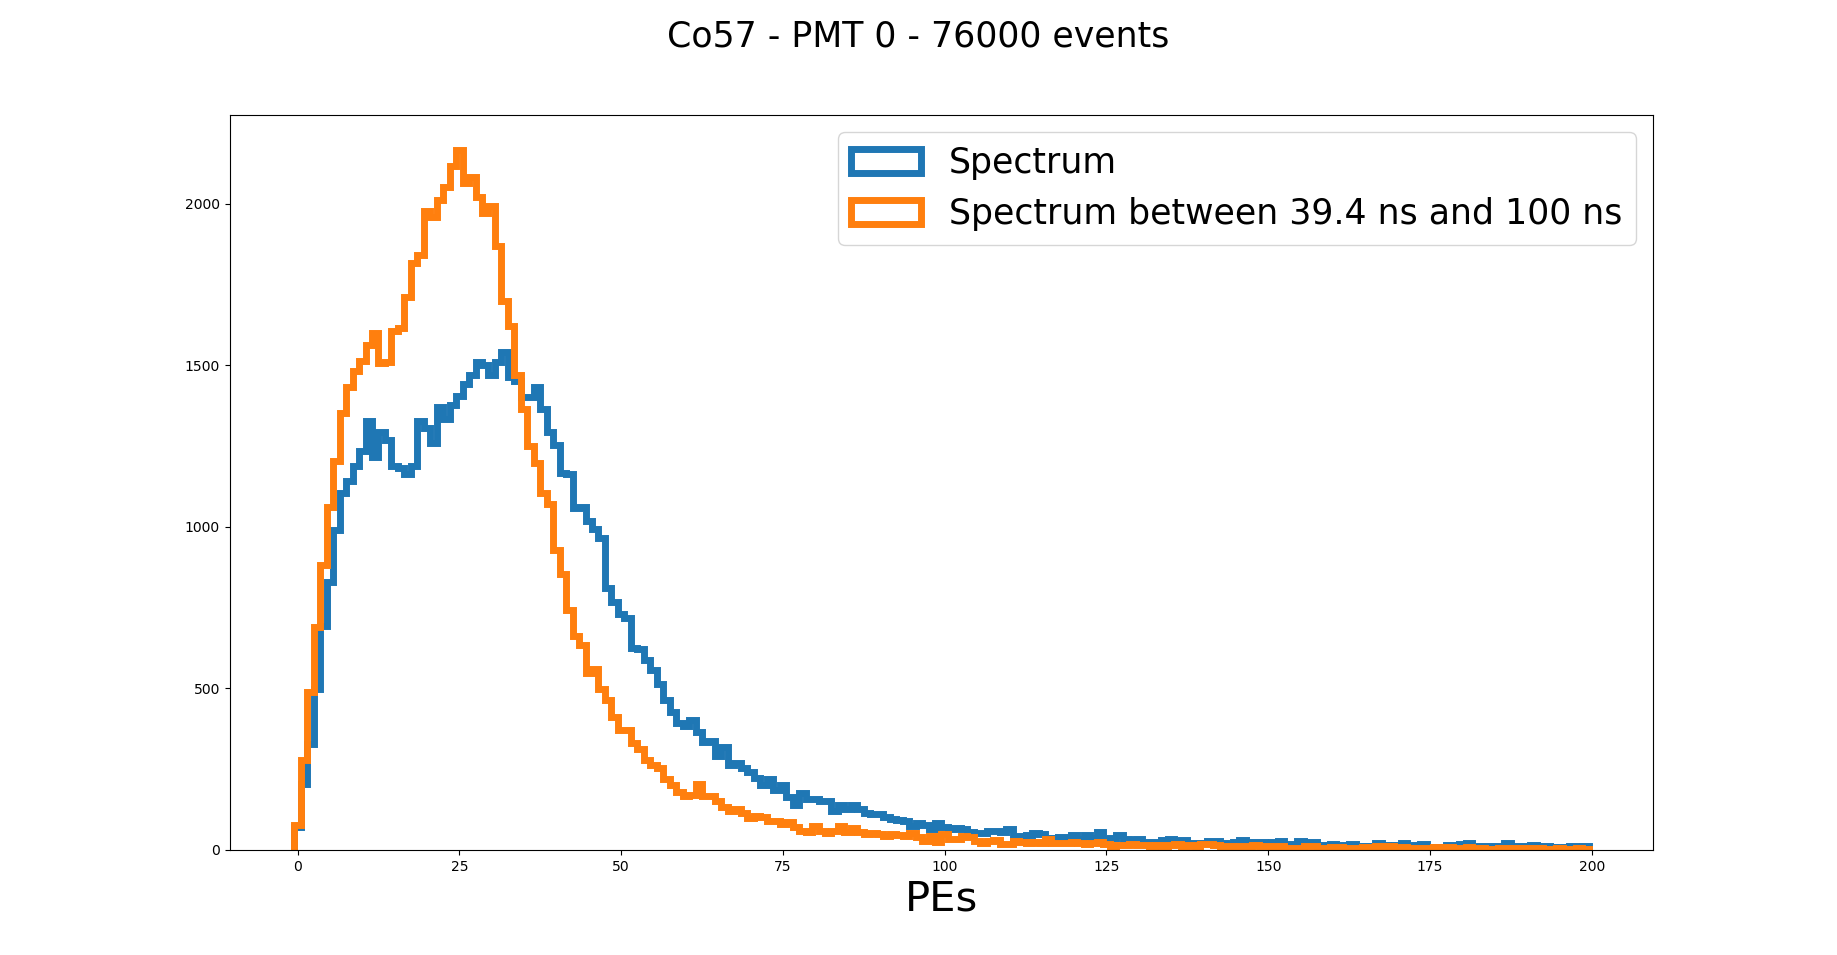
\includegraphics[width=1\linewidth]{SpecCo0.png}
\end{figure}
\end{frame}

\begin{frame}
\begin{figure}[h]
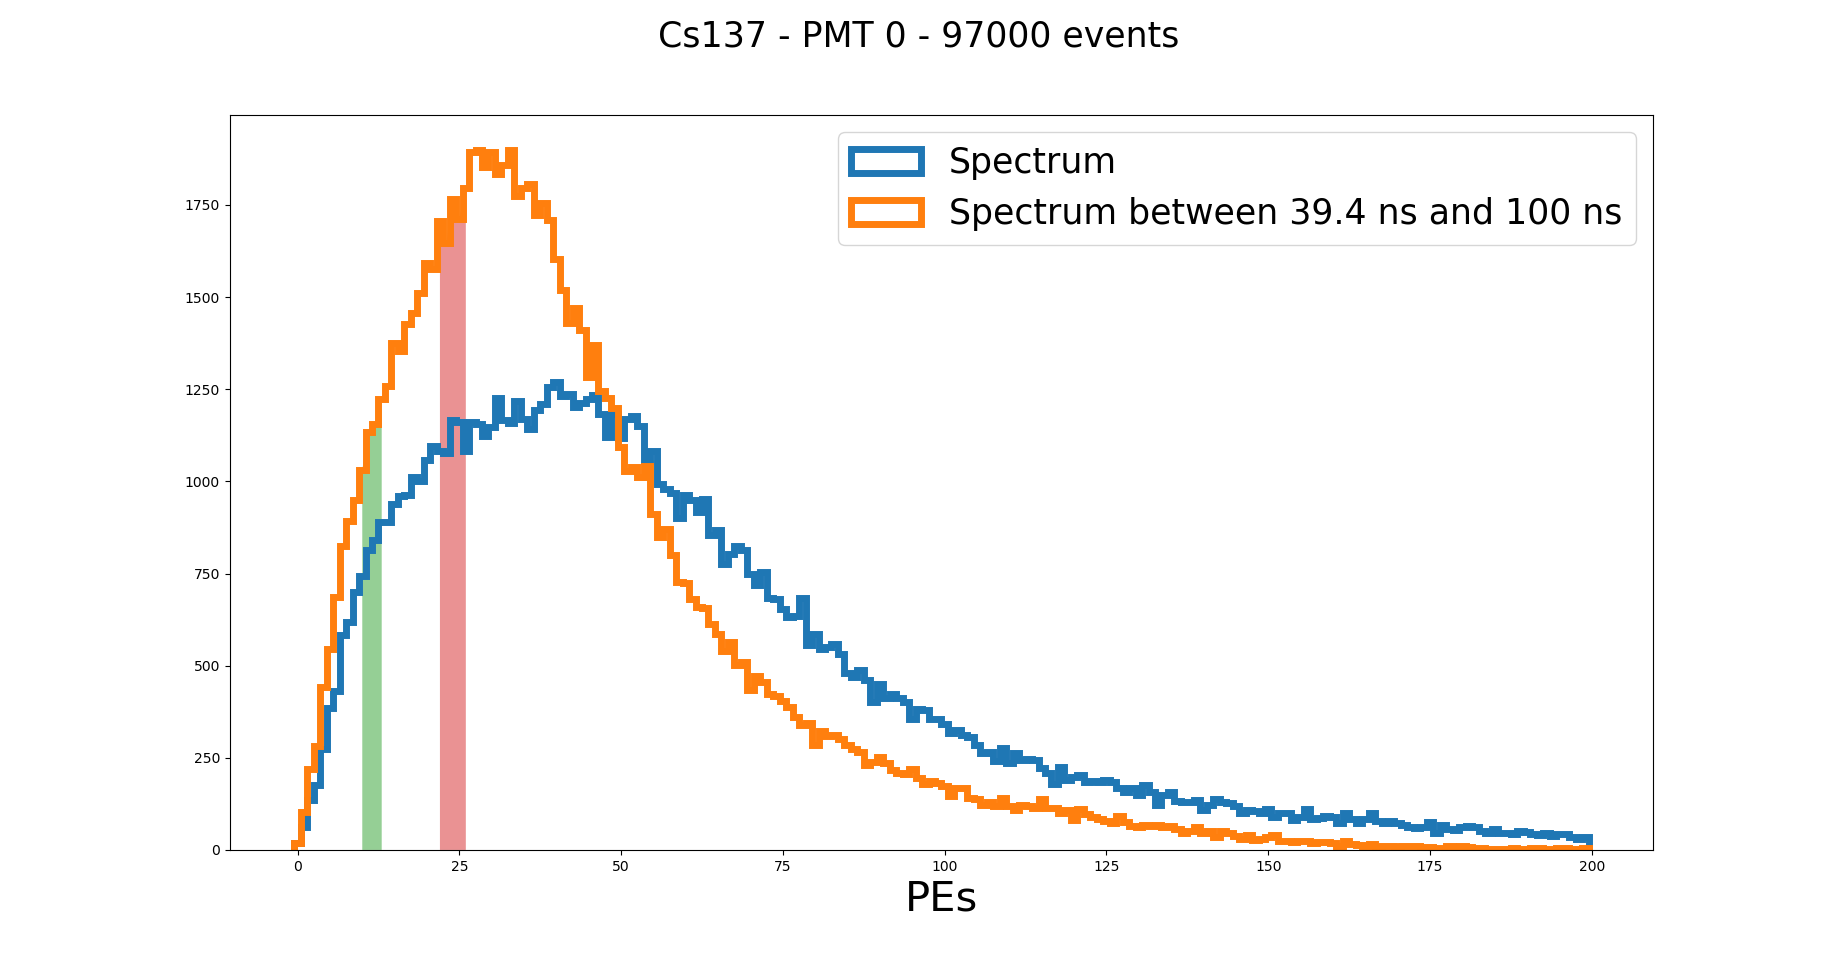
\includegraphics[width=1\linewidth]{SpecCs0.png}
\end{figure}
\end{frame}

\begin{frame}
\begin{figure}[h]
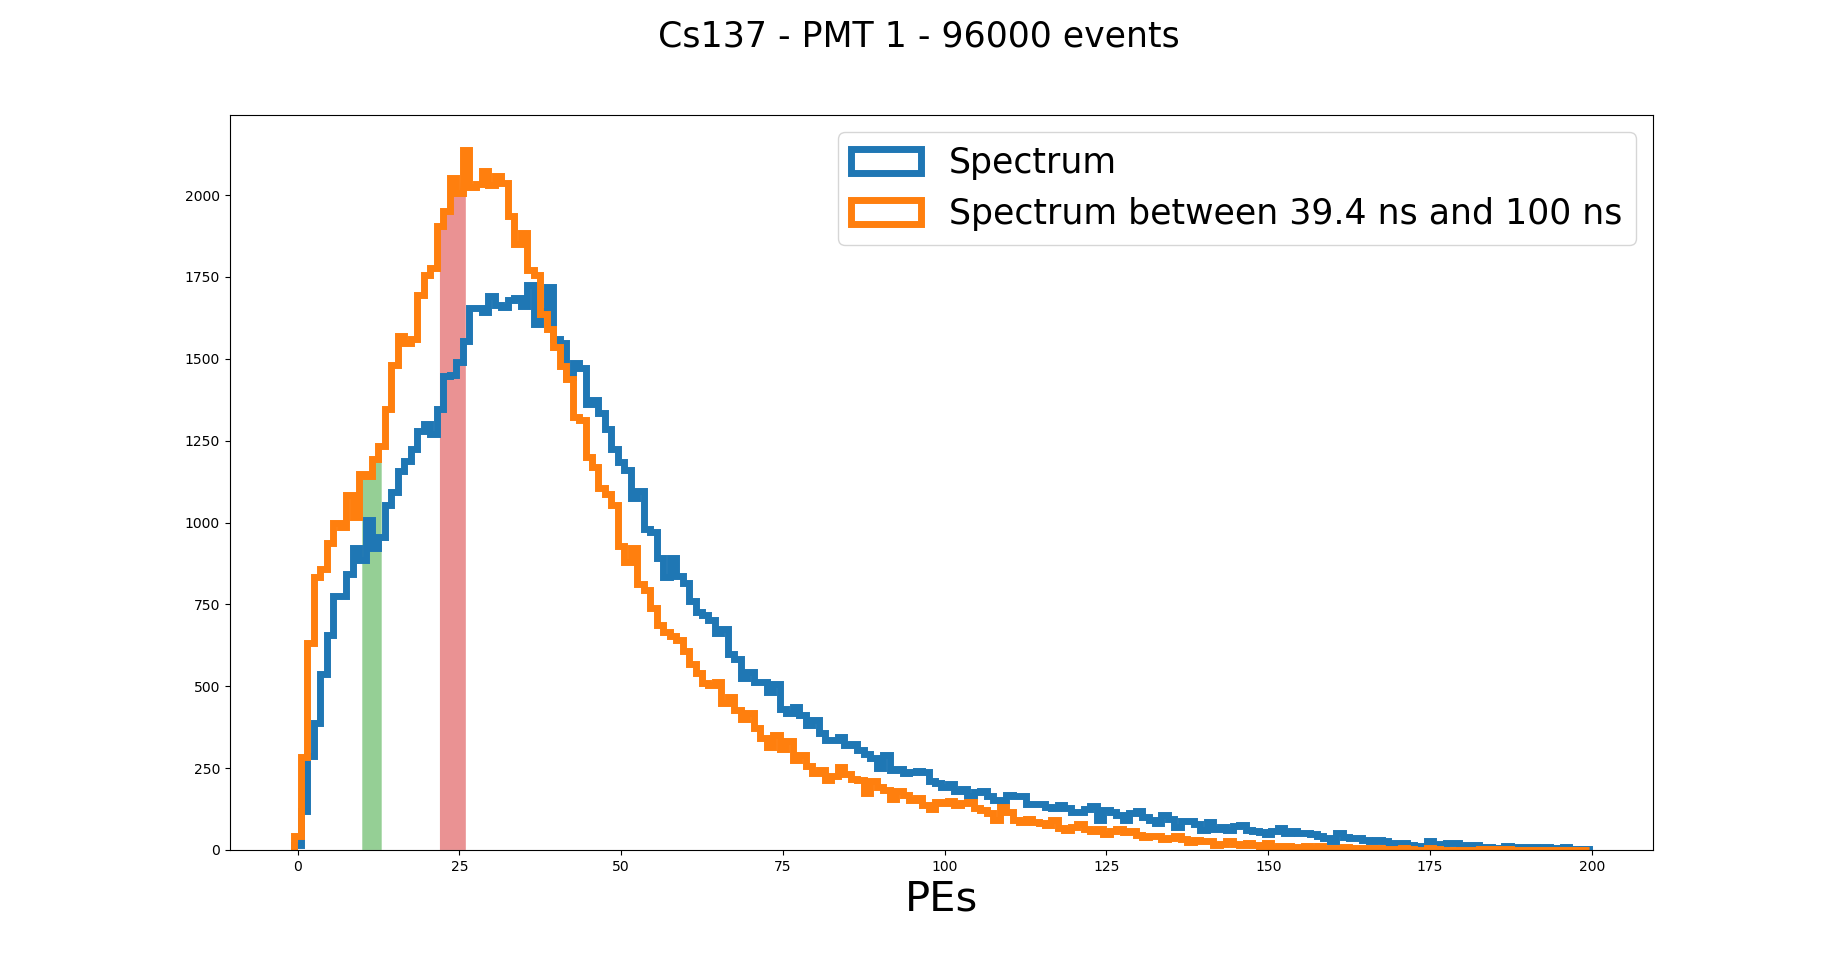
\includegraphics[width=1\linewidth]{SpecCs1.png}
\end{figure}
\end{frame}

\begin{frame}
\begin{figure}[h]
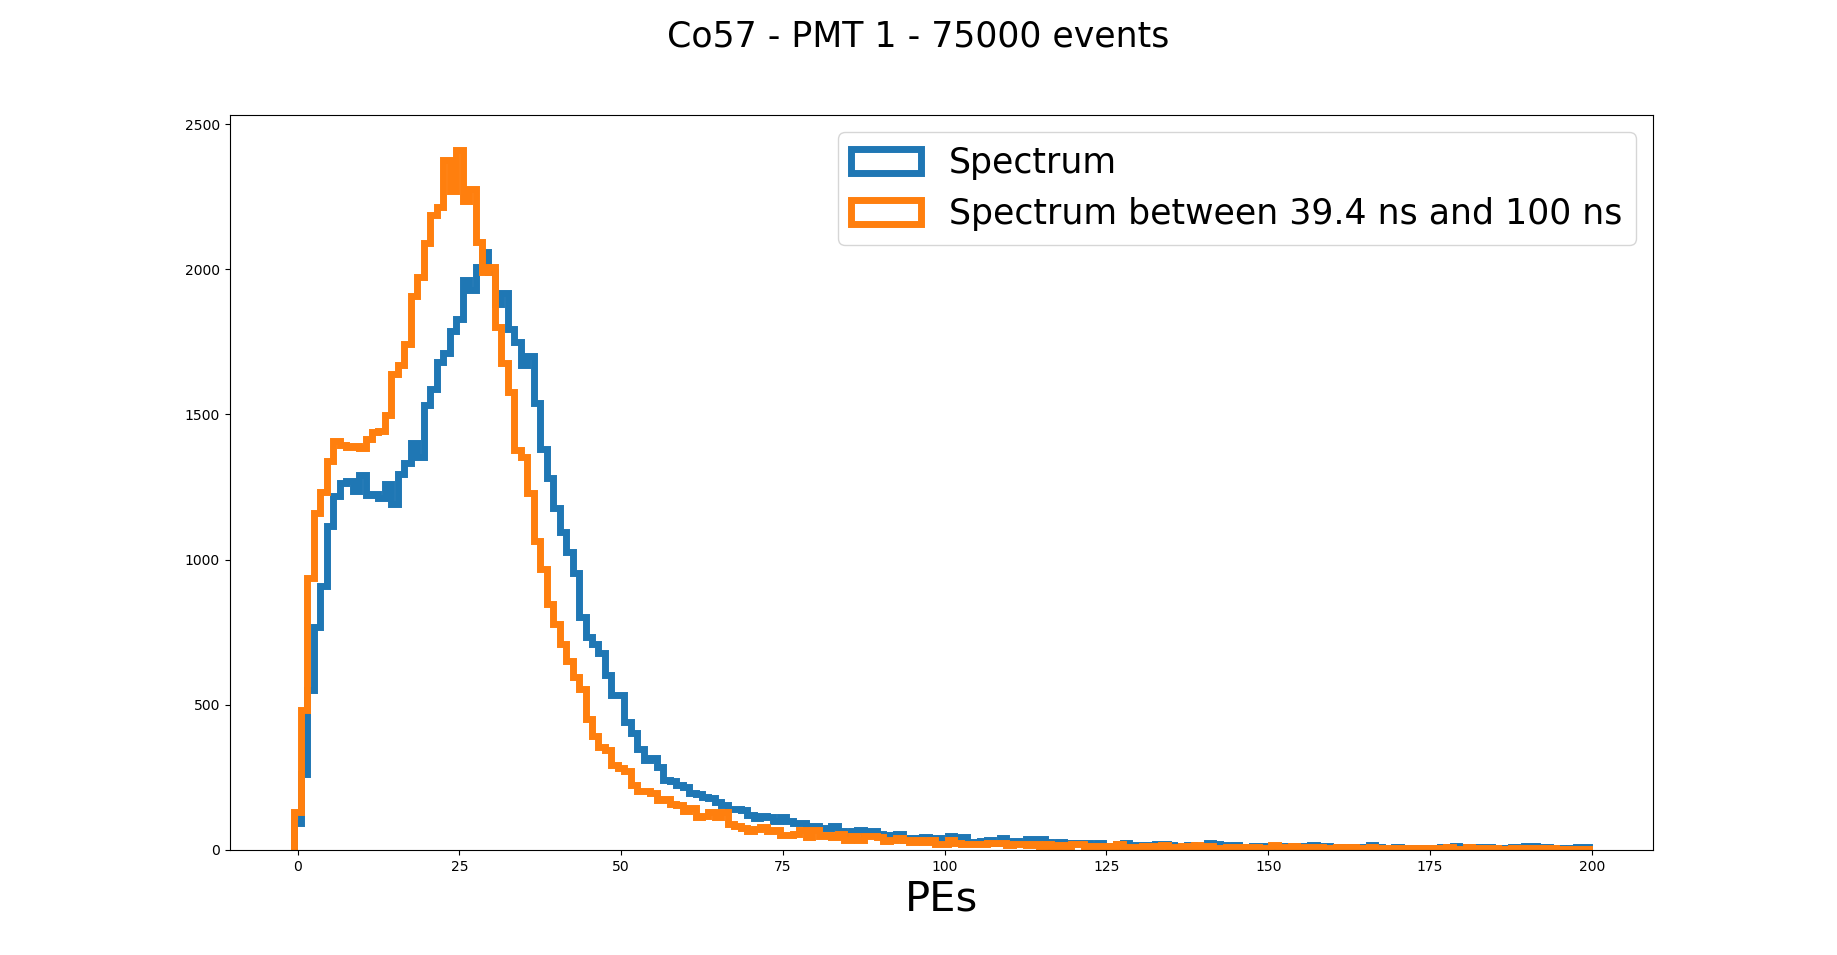
\includegraphics[width=1\linewidth]{SpecCo1.png}
\end{figure}
\end{frame}

\begin{frame}
\begin{figure}[h]
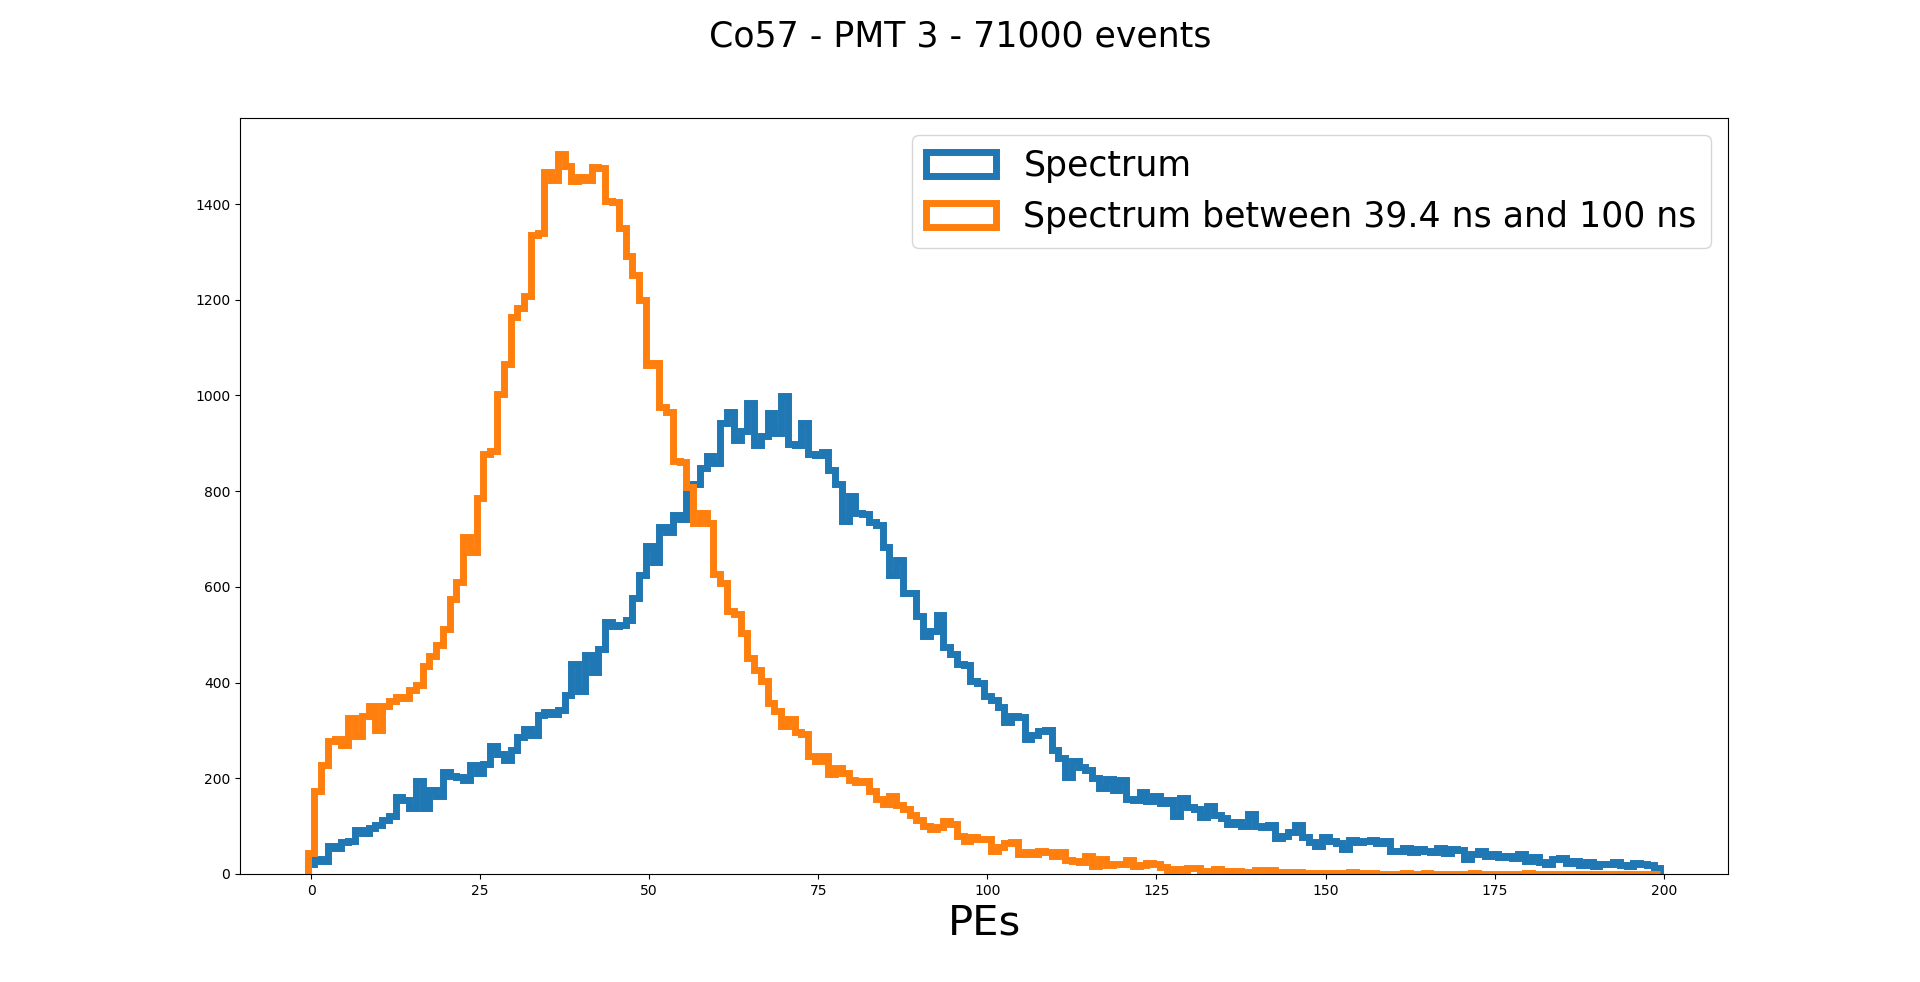
\includegraphics[width=1\linewidth]{SpecCo3.png}
\end{figure}
\end{frame}

\begin{frame}
\begin{figure}[h]
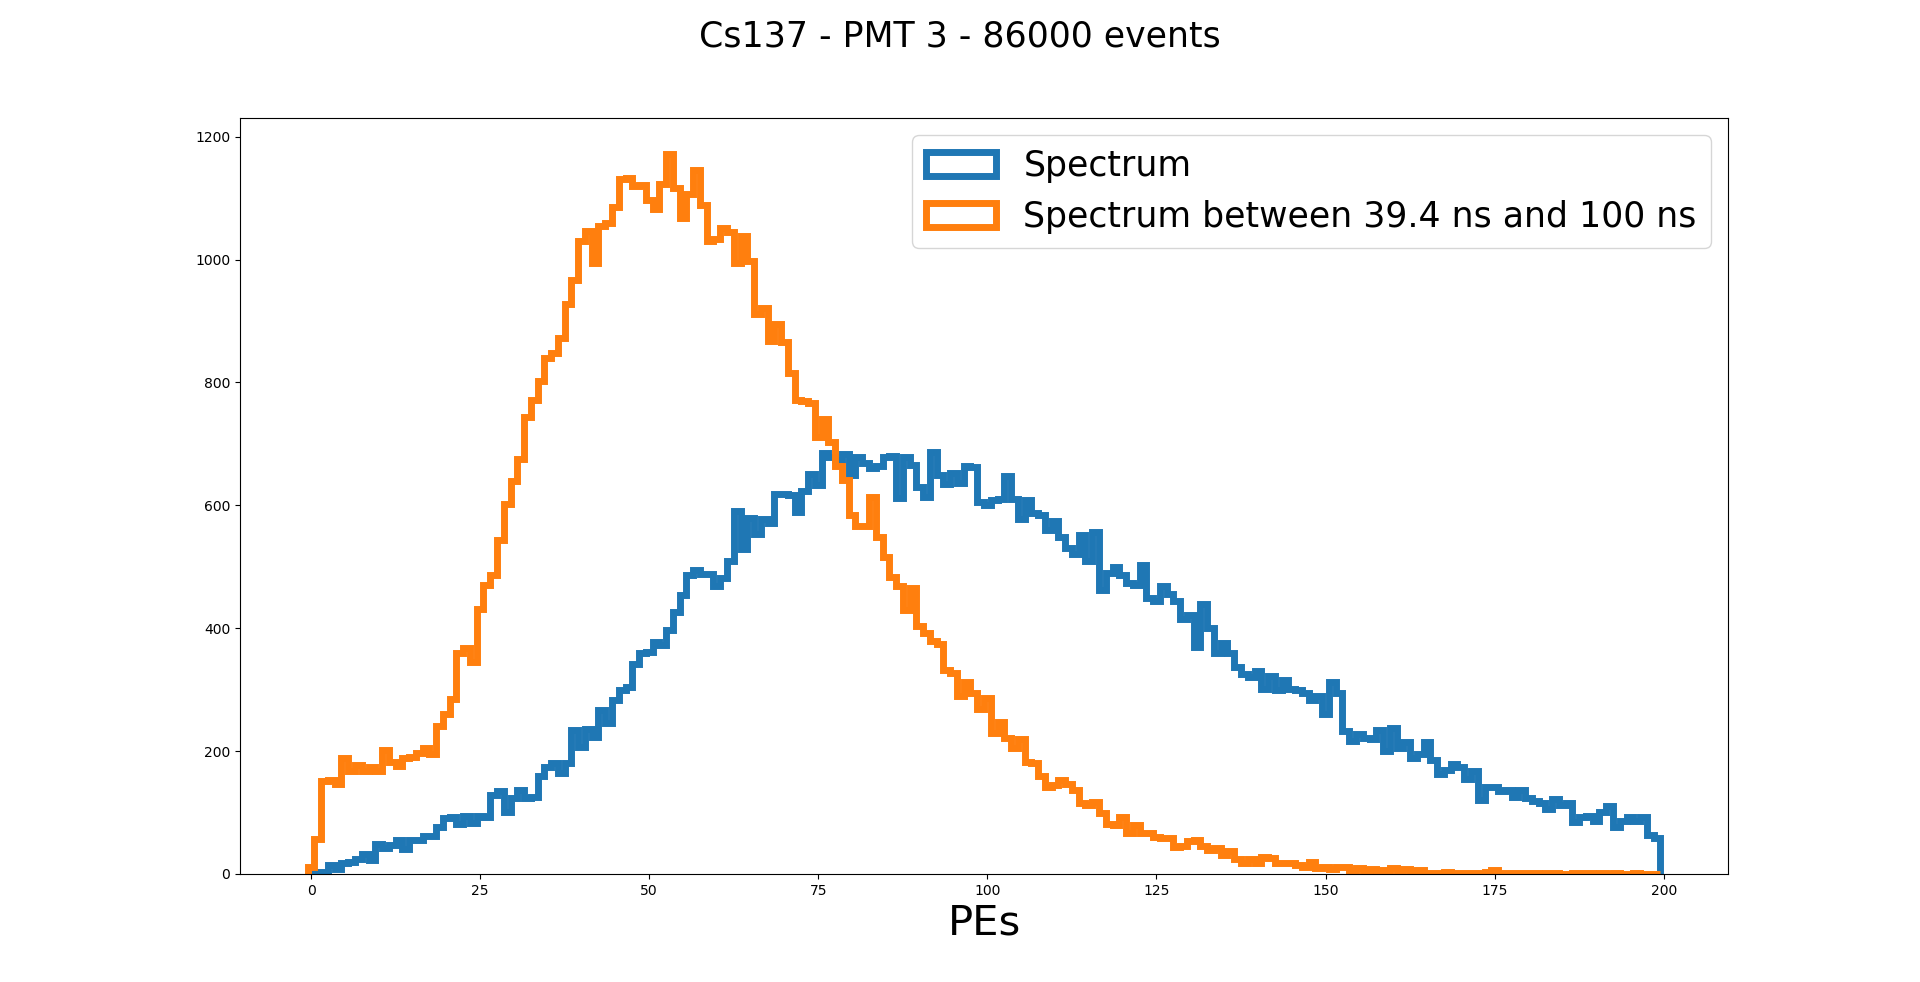
\includegraphics[width=1\linewidth]{SpecCs3.png}
\end{figure}
\end{frame}

\begin{frame}{PE Histogram}
The basis for analysis is a 2D histogram (for each PMT and each source) $H_{ni}$ which holds the number of events in which $n$ PEs were resolved at time $i$,
\begin{figure}[h]
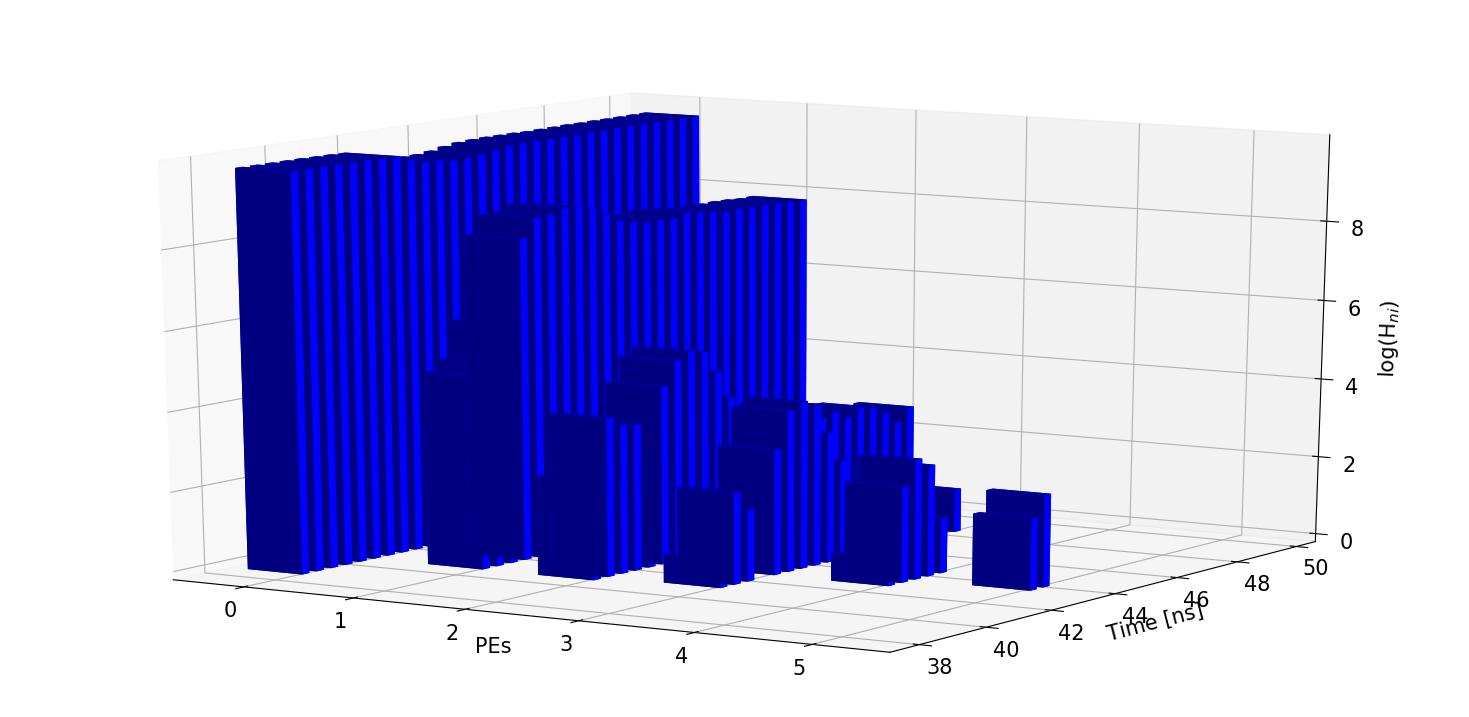
\includegraphics[width=0.9\linewidth]{H.png}
\end{figure}
The average temporal structure which shown in the Reconstruction result slide is the average on each column.
\end{frame}


\begin{frame}{Model for $H_{ni}$}
The number of photons emitted at time $i$,
\begin{equation}
n_i^{ph}\sim \text{Poisson}(Y_iN),
\end{equation}
where $N$ is the average number of photon emitted in the events, and $Y_i$ is the scintillation model (the probability to emit a photon at time $i$).\\
The number of PEs created in the PMT at time $i$,
\begin{equation}
n_i^{pe}\sim \text{Binom}(Q, \text{Poisson}(Y_iN)),
\end{equation}
where $Q$ is the photon detection efficiency (quantum efficiency, collection efficiency and double PE probability).
\end{frame}

\begin{frame}
Each PMT has its temporal uncertainty combined with the code's temporal uncertainty. The number of PEs that need to be resolved at time $i$,
\begin{equation}
\tilde n_i\sim \sum_j m_j^i,
\end{equation}
where $m_j^i$ is a random variable that represents the number of PEs that were created at time $j$ but resolved at time $i$.  

\begin{equation}
m_j^i\sim n_j^{pe}\text{Norm}(i-j-T|\sigma_t)
\end{equation}
where $\sigma_t$ is the temporal resolution of the PMT and the code and $T$ is the average delay of the PMT.
\end{frame}

\begin{frame}
Since $\tilde n_i$ is a sum of independent random variables its distribution can be approximated by a distribution with mean and variance $\langle\tilde{n}_i\rangle=\sum_j\langle m\rangle_j^i$, Var$_i=\sum_j$Var$_j^i$,
where, 
\begin{equation}
\langle m\rangle_j^i=\text{Var}_j=QN_0Y_j\text{Norm}(i-j-T|\sigma_t)
\end{equation}

Poisson has an equal mean and variance, so 
\begin{equation}
\tilde{n_i}\sim \text{Poisson}\left(QN\sum_jY_j\text{Norm}(i-j-T|\sigma_t)\right)
\end{equation}
\end{frame}

\begin{frame}{Scintillation model}
$Y_j$ is the probability to emit a photon at time $t_j\Delta t$.\\
\begin{equation}
Y_j=\Delta tF\delta(t_j-T)+\Delta t\frac{1-F}{\tau_s}e^{-t_j/\tau_s}
\end{equation}
\begin{equation}
\begin{split}
&\langle \tilde{n_i}\rangle=\frac{QN\Delta t}{\sqrt{2\pi}\sigma_t}\int_0^{\infty}Y(\tilde{t})e^{-(\tilde{t}-t_i-T)^2/2\sigma_t^2}=\\
&NQ\Delta t\left[\frac{e^{-(t_i-T)^2/2\sigma_t^2}}{\sqrt{2\pi}\sigma_t}+\frac{K}{\tau}e^{-t/\tau}\left(1-\text{erf}\left(\frac{\sigma}{\sqrt{2}\tau}-\frac{t-T}{\sqrt{2}\sigma}\right)\right)\right]
\end{split}
\end{equation}
Where $K$ is a normalization constant,
\begin{equation}
K=\left[1-\text{erf}\left(\frac{\sigma}{\sqrt{2}\tau}+\frac{T}{\sqrt{2}\sigma}\right)+e^{-\sigma^2/2\tau^2-T/\tau}\left(1+\text{erf}\left(\frac{T}{\sqrt{2}\sigma}\right)\right)\right]^{-1}
\end{equation}
\end{frame}

\begin{frame}{SPE resolution}
Finally, the code has its resolution for SPEs (its accuracy to resolve the correct number of PEs from the signal at a given time). The probability to resolve $n$ PEs given $\tilde{n}$ is the correct number,
\begin{equation}
n_i\sim \text{P}_{n}(\tilde n|\sigma_{pe})=\sum_{m}\text{Norm}(m-1|\sigma_{pe})\text{P}_{n-m}(\tilde{n}-1|\sigma_{pe})
\end{equation}
\end{frame}

\begin{frame}{Expectation for $H_{ni}$}
The expected number of events in which $n$ PEs were resolved at time $i$ is,
\begin{equation}
h_{ni}=N_{ev}\sum_{m}\text{P}_n(m|\sigma_{pe})\text{Poisson}(m|\langle \tilde{n}_i\rangle)
\end{equation}
This is a model with 7 parameters: $N, Q, F, \tau_s, T, \sigma_t, \sigma_{PE}$. Some of them can be constrained by calibration data.
\end{frame}

\begin{frame}{Calibration $\sigma_t$}
We can calibrate $\sigma_t$ for each PMT by the pulser data. Consider PMT$_i$ that we want to calibrate and a any other PMT$_j$. For each pulser event in which both PMTs saw SPE we measure $\Delta_{ij}$, the time difference between the two signals. $\Delta_{ij}\sim\text{Norm}(T_{ij}, \sigma_{ij})$.
\begin{figure}[h]
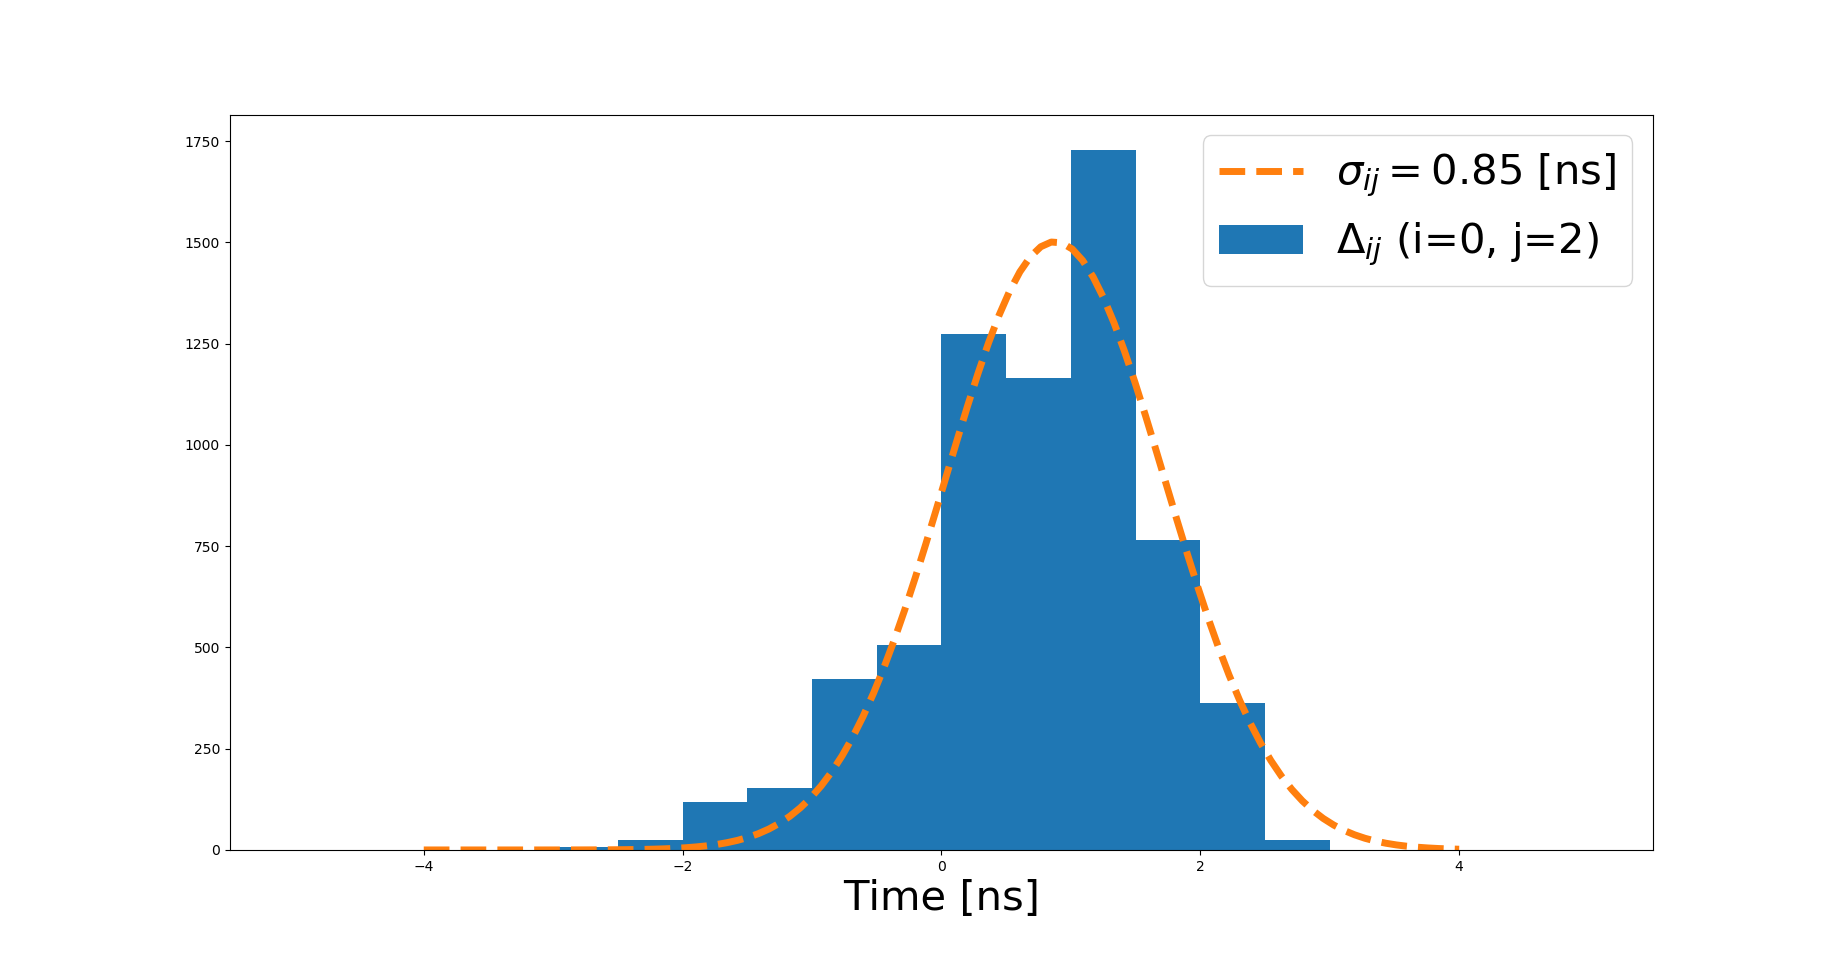
\includegraphics[width=1\linewidth]{sigma_ij.png}
\end{figure}
\end{frame}

\begin{frame}
$\sigma_i=\sqrt{\frac{1}{2}(\sigma^2_{ij}+\sigma^2_{ik}-\sigma^2_{jk})}$ for any $j\neq k$.\\
So a pair of PMTs ($k,j$) is used to estimate the $\sigma_i$. Each PMT$_i$ has $\frac{1}{2}{19\choose 2}$ estimates for $\sigma_i$ and their mean is $\sigma_t$ for that PMT.
\begin{figure}[h]
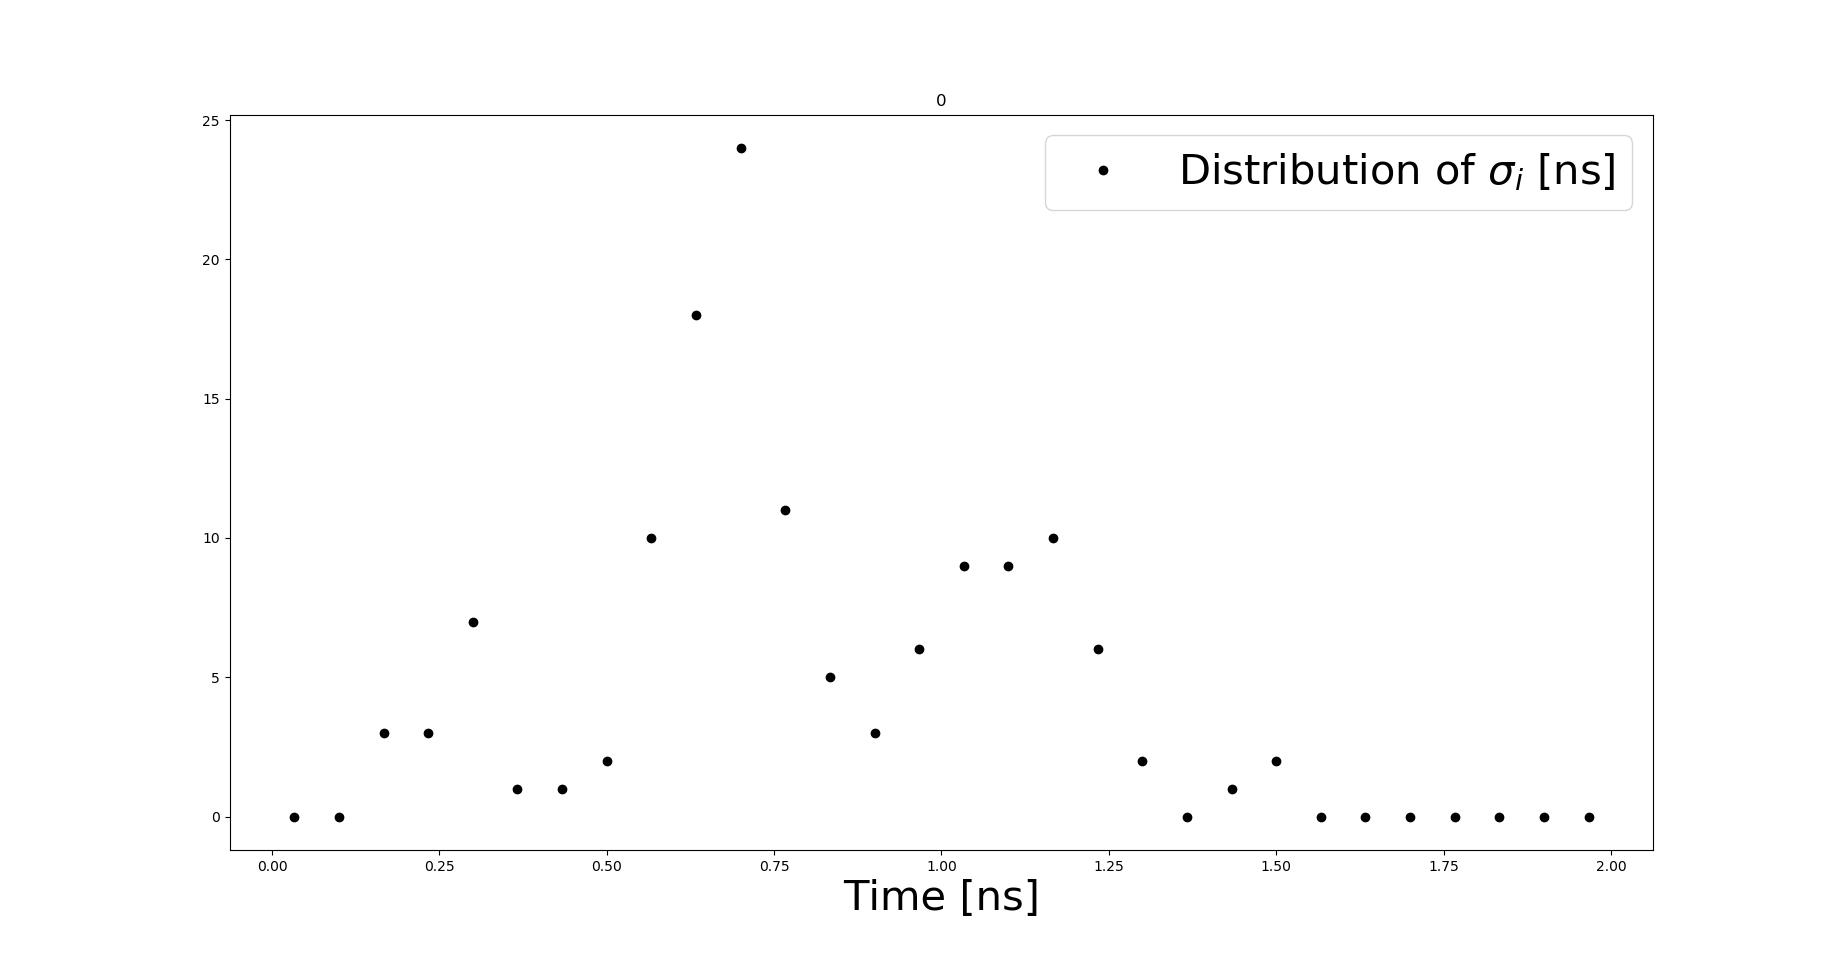
\includegraphics[width=1\linewidth]{sigma_i.png}
\end{figure}
\end{frame}

\begin{frame}{Calibration of $\sigma_{PE}$}
$\sigma_{PE}$ is the standard deviation of the distribution of the number of PEs that are resolved from a SPE created in the PMT. This is calibrated from the SPE area distribution.
\begin{equation}
\text{Area}_{spe}\sim\text{Norm}(\bar{A}, \bar{A}\cdot\sigma_{PE})\quad \rightarrow \quad n\sim\text{Norm}(1,\sigma_{PE})
\end{equation}
\begin{figure}[h]
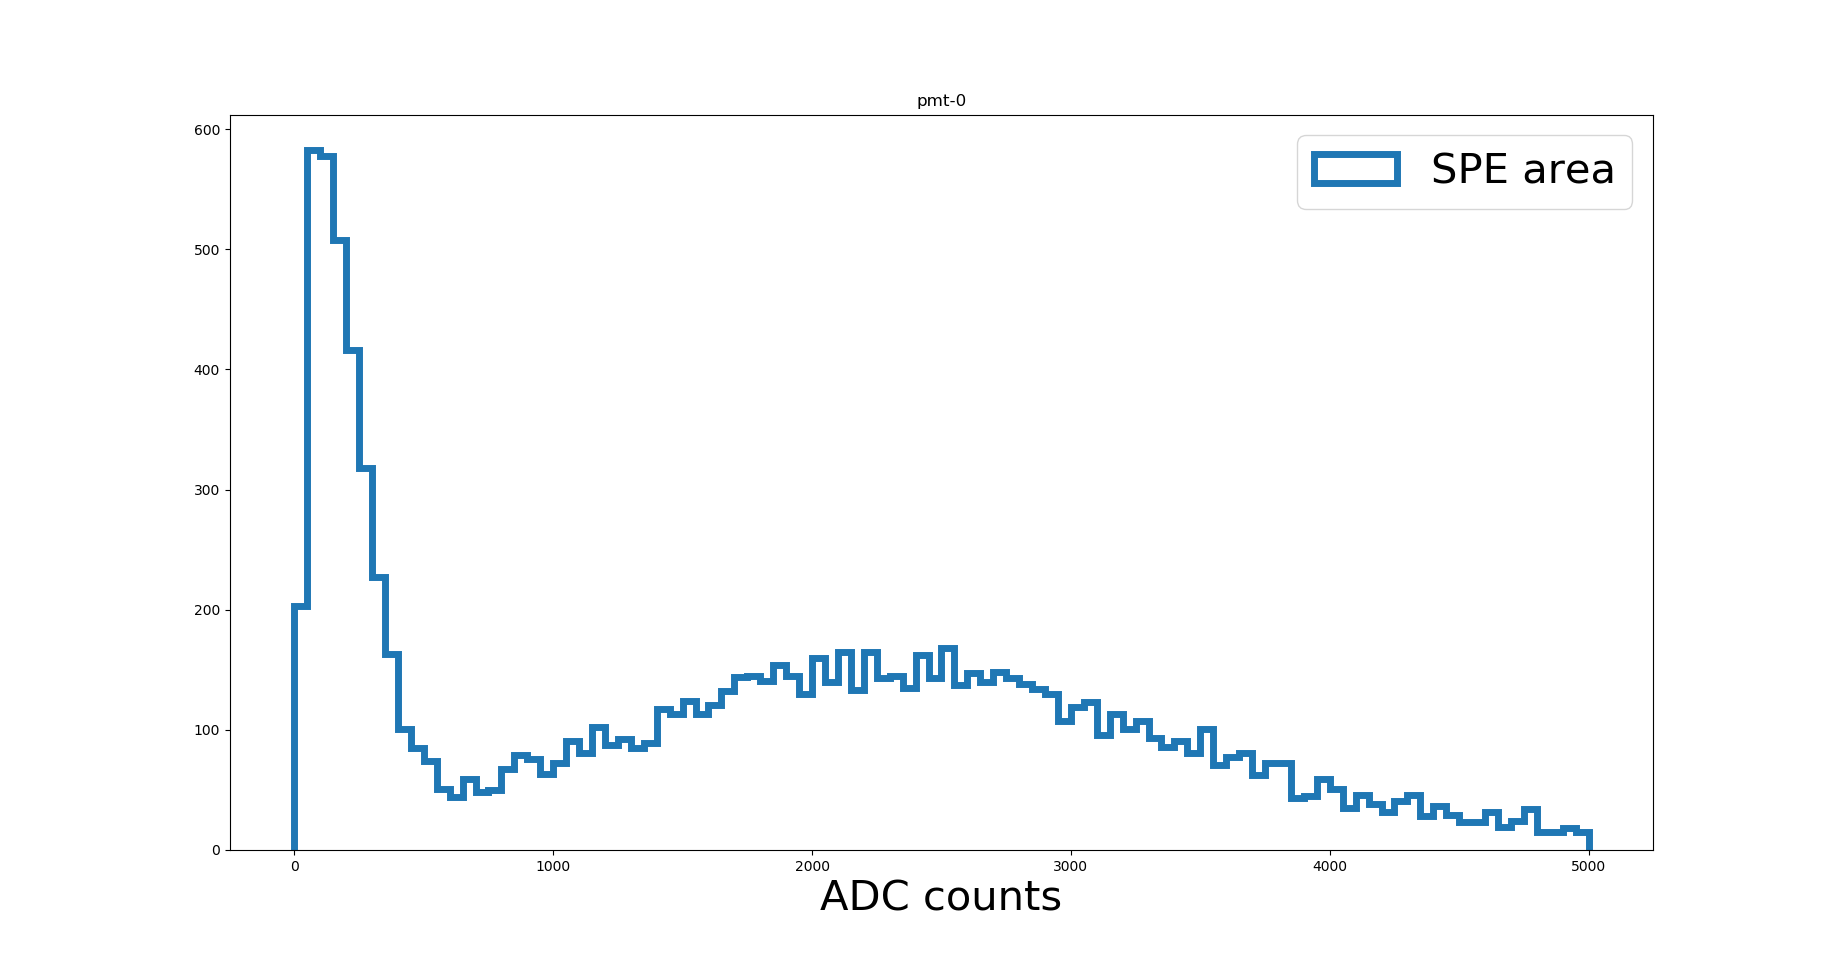
\includegraphics[width=1\linewidth]{area.png}
\end{figure}
\end{frame}

\begin{frame}{Constrain on $NQ$}
We choose the data to fit our model to from a narrow PE bands in the spectrum, where it can be estimated that the origin of the events in these bands is from the same energy and their variation is due to statistical fluctuation and no physical. Thus we expect that
\begin{equation}
N_{PE}\sim\text{Poisson}(\sum_{39.4 ns}^{100 ns}\langle h_{ni}\rangle_n)
\end{equation}  
\begin{figure}[h]
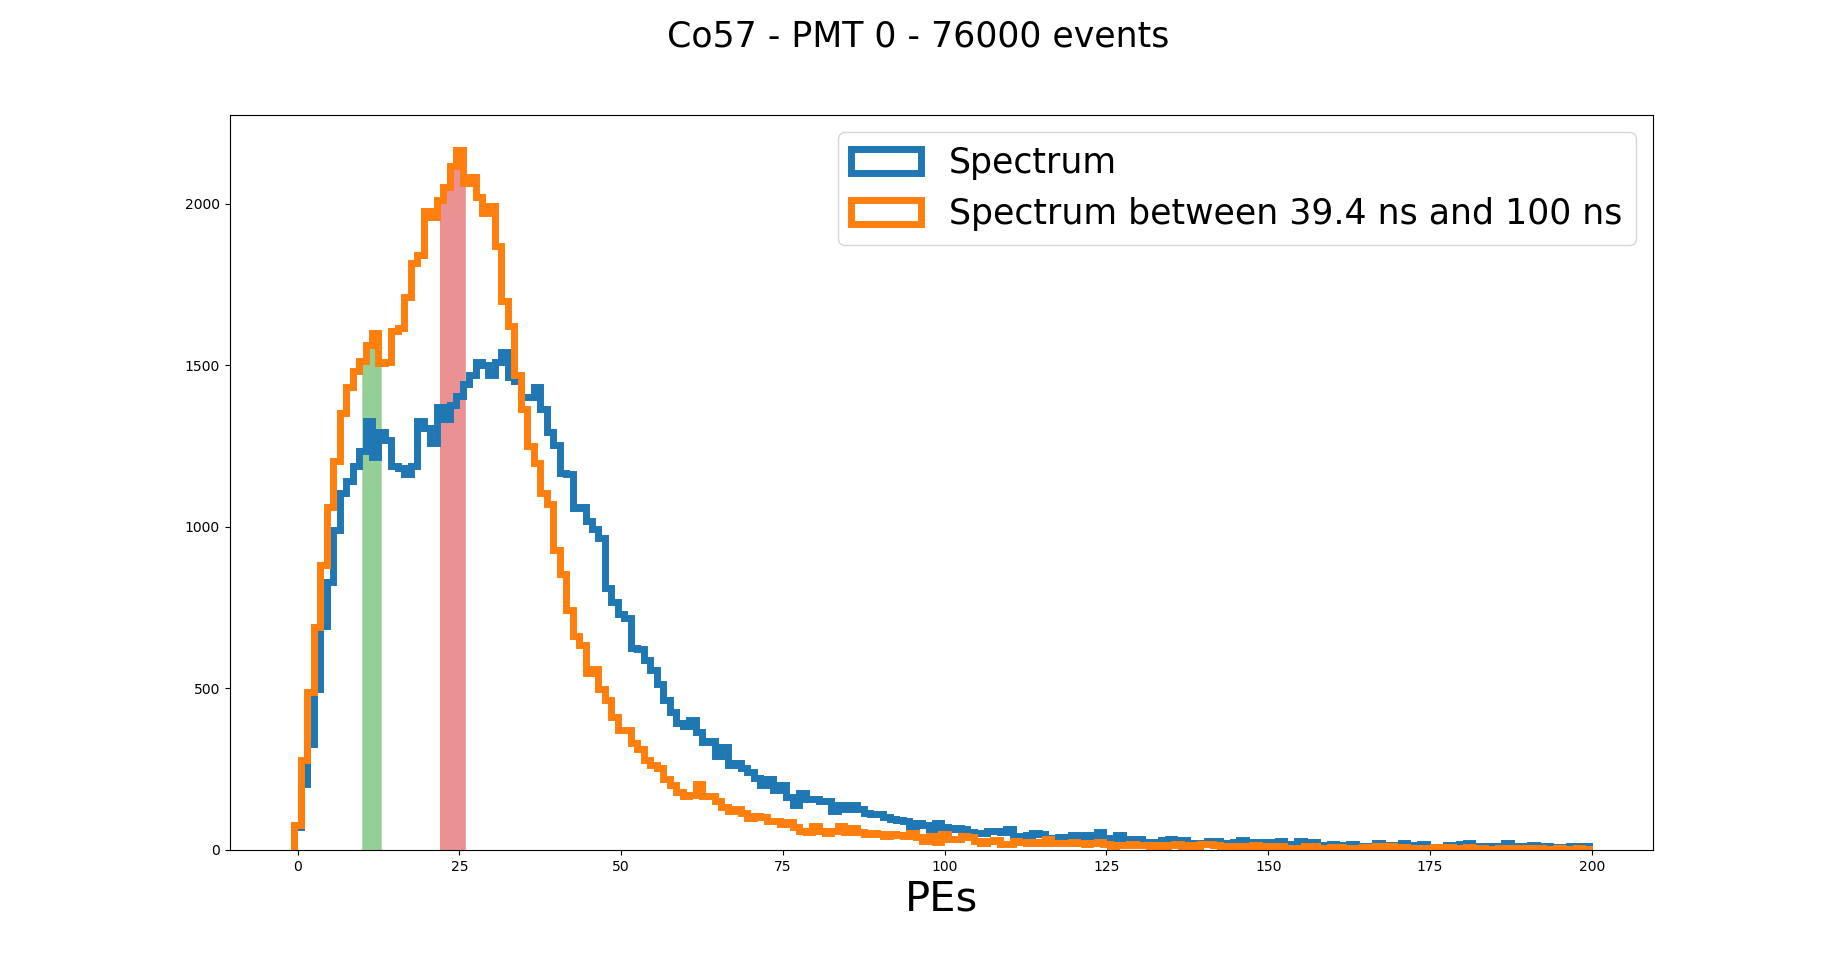
\includegraphics[width=0.75\linewidth]{spec_peak.png}
\end{figure}
\end{frame}

\begin{frame}{Fit}
To find the parameters which give $h_{ni}$ as close to $H_{ni}$ we maximize 
\begin{equation}
L(\text{data},\text{model}(\theta))=\sum_{\text{dataset}}\sum_{j\in J}\text{Poisson}(\text{data}_j|\text{model}_j)/\text{len}(J)
\end{equation}
Where $\theta$ is the parameter array and $J$ is some sub-range of the dataset. The datasets in the summation:
\begin{itemize}
\item Dataset - $H_{ni}$, model - $h_{ni}$.
\item Dataset - distribution of estimates for $\sigma_t$, model - Norm($\sigma_t, \Sigma_t$).
\item Dataset - distribution of SPE areas, model - Norm($\bar{A}, \bar{A}\cdot\sigma_{PE}$).
\item Dataset - PE spectrum, model - $\text{Poisson}(\sum_{39.4 ns}^{100 ns}\langle h_{ni}\rangle_n)$.
\end{itemize}
This adds two dummy parameters, $\Sigma_t$ is the standard deviation of the estimates of $\sigma_t$ and $\bar{A}$ is the mean SPE area. 
\end{frame}

\begin{frame}{Results ($^{57}$Co peak 2)}
\begin{figure}[h]
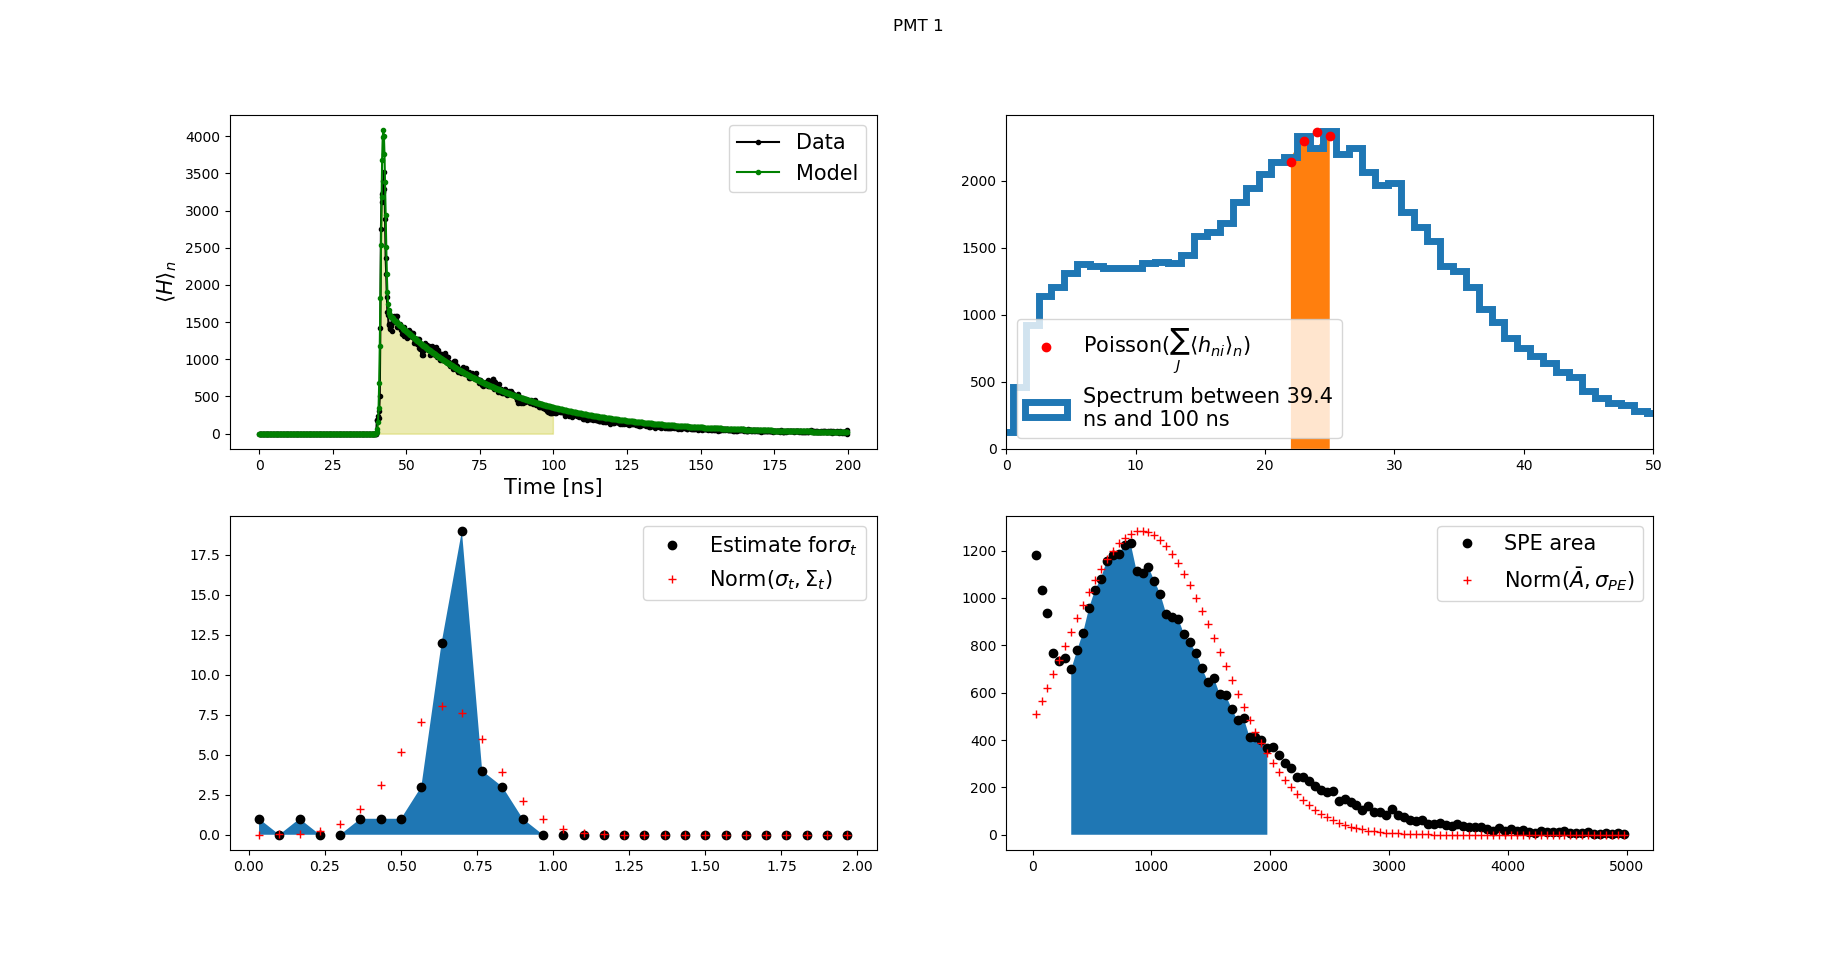
\includegraphics[width=1\linewidth]{Co2.png}
\end{figure}

\begin{center}
\begin{tabular}{ |c| c| c| c| c|}
\hline
 $NQ$ & $F$ & $\sigma_t [ns]$ & $\sigma_t [ns]$ & $\sigma_{PE}$\\ 
\hline
33 & 0.1 & 34 & 0.6 & 0.7\\  
\hline   
\end{tabular}
\end{center}
\end{frame}


\begin{frame}{Results ($^{137}$Cs)}
\begin{figure}[h]
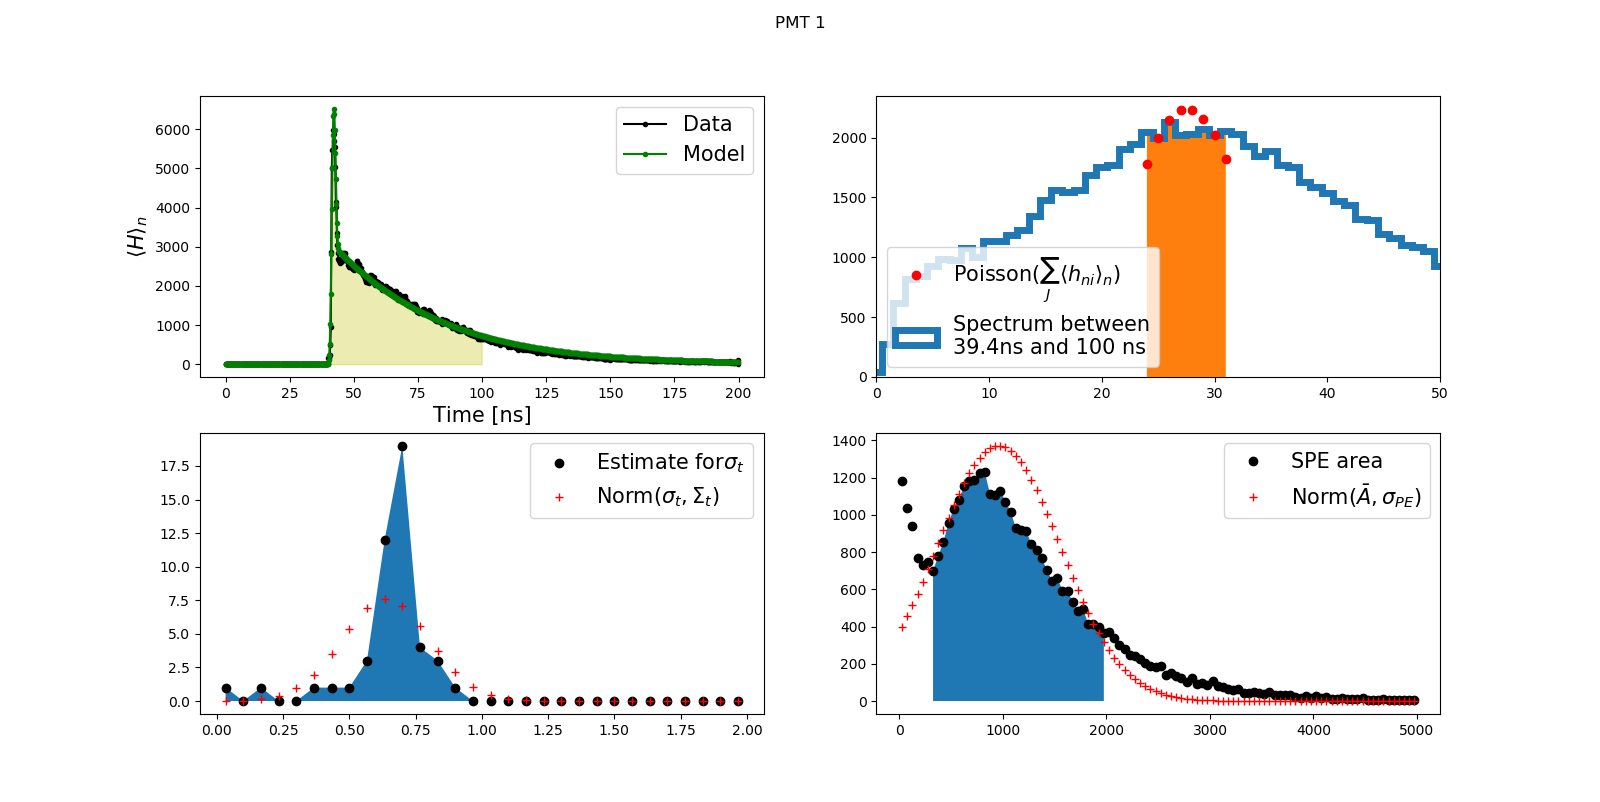
\includegraphics[width=1\linewidth]{Cs.png}
\end{figure}

\begin{center}
\begin{tabular}{ |c| c| c| c| c|}
\hline
 $NQ$ & $F$ & $\sigma_t [ns]$ & $\sigma_t [ns]$ & $\sigma_{PE}$\\ 
\hline
39 & 0.09 & 38 & 0.6 & 0.6\\  
\hline   
\end{tabular}
\end{center}
\end{frame}

\begin{frame}{Results ($^{57}$Co peak 1)}
Notice that for this peak $F$ is much greater and $\tau_s$ is much smaller.
\begin{figure}[h]
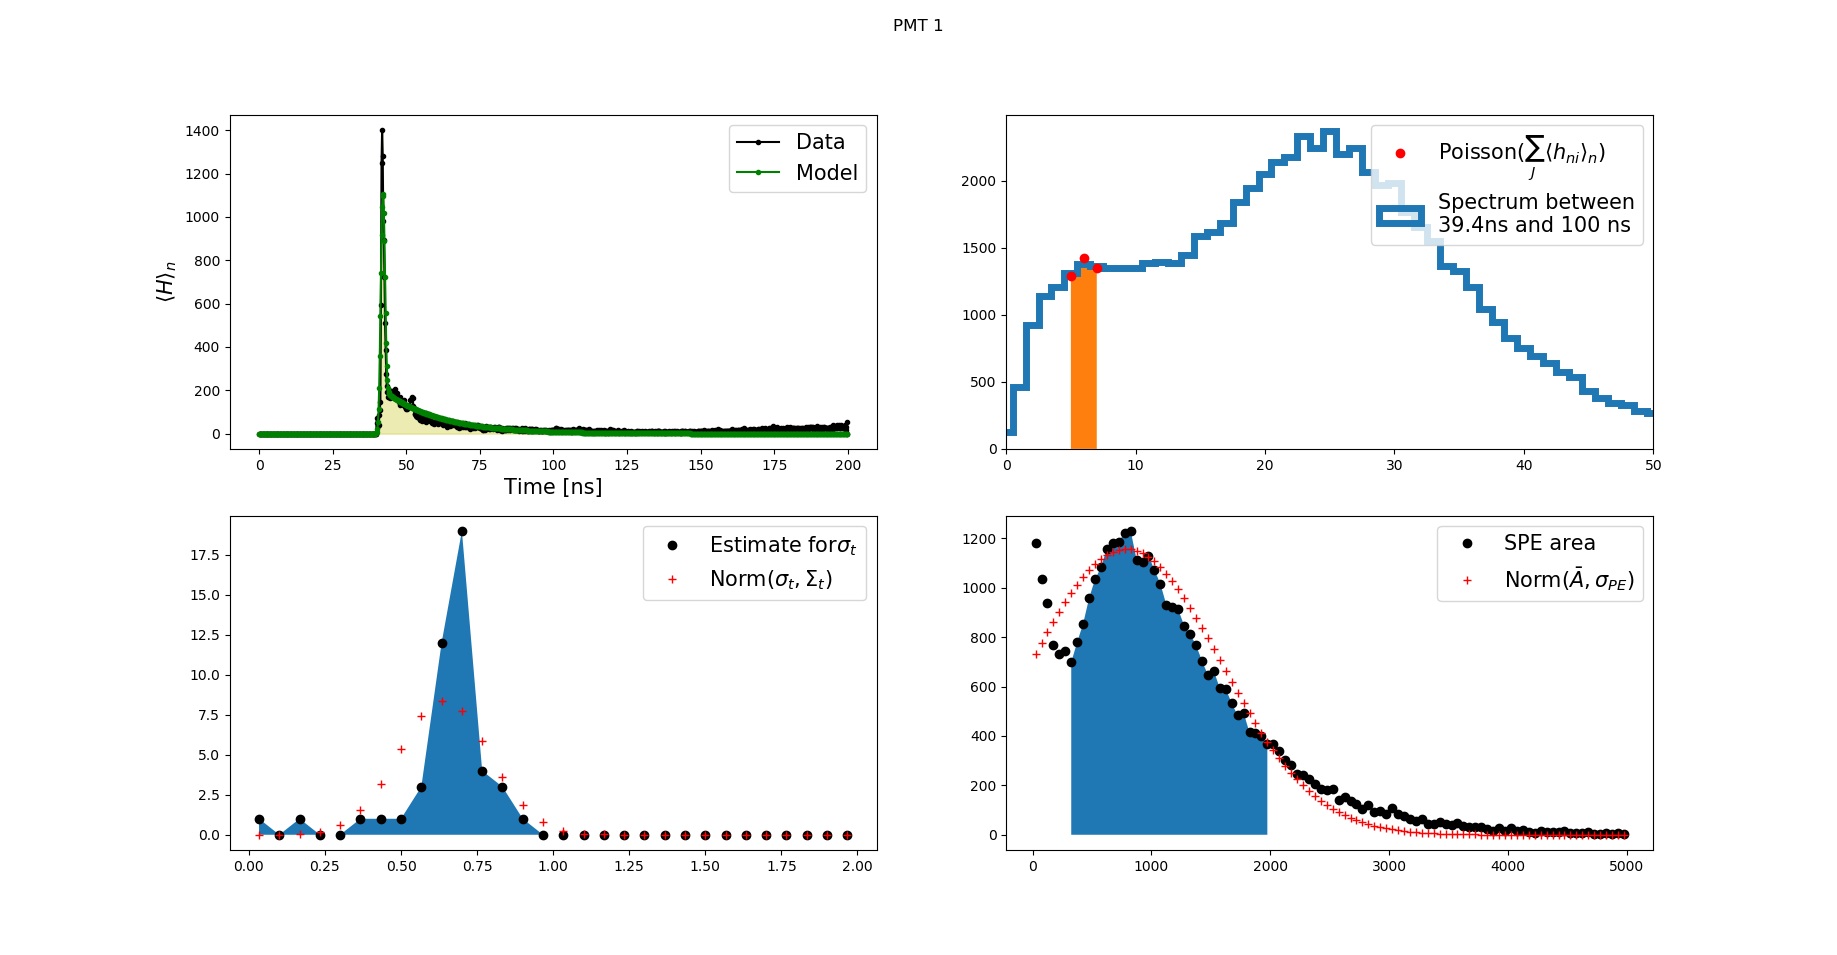
\includegraphics[width=1\linewidth]{Co1.png}
\end{figure}

\begin{center}
\begin{tabular}{ |c| c| c| c| c|}
\hline
 $NQ$ & $F$ & $\sigma_t [ns]$ & $\sigma_t [ns]$ & $\sigma_{PE}$\\ 
\hline
7 & 0.4 & 18 & 0.6 & 1\\  
\hline   
\end{tabular}
\end{center}
\end{frame}

\begin{frame}{Results ($^{57}$Co peak 1 - strange result)}
\begin{figure}[h]
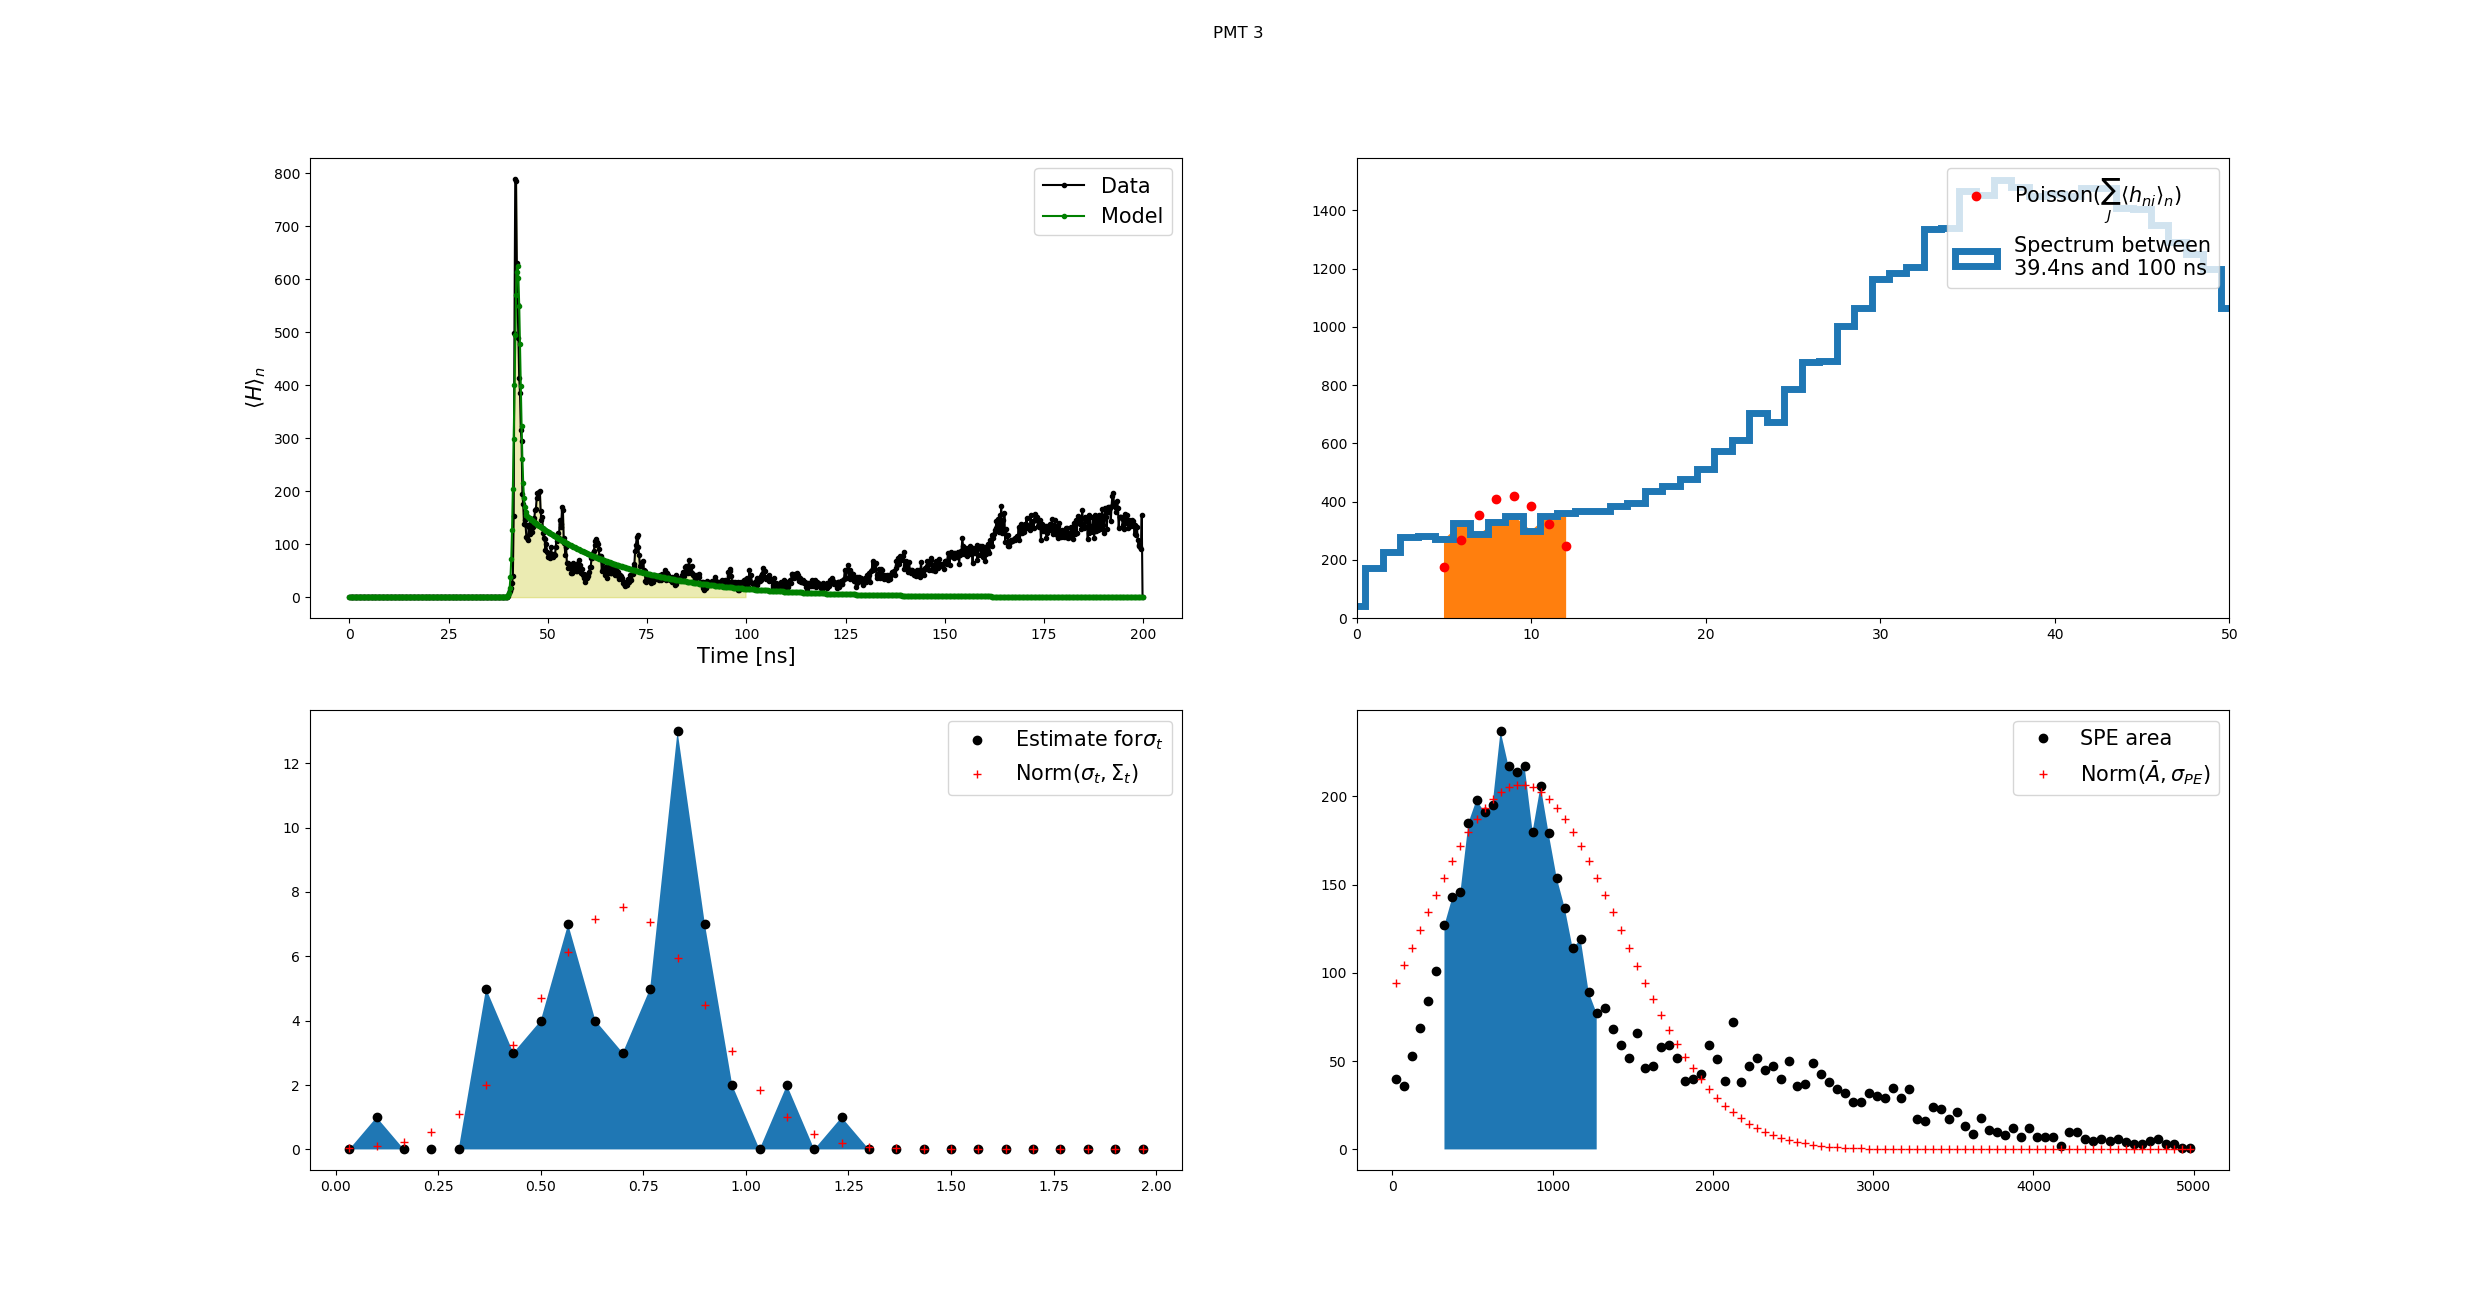
\includegraphics[width=1\linewidth]{wird.png}
\end{figure}
\end{frame}

\begin{frame}{Parameter estimation}
$\hat{\theta}$ is the parameter array that maximize $L$, so for any parameter $\theta_i$, 
\begin{equation}
\begin{split}
\partial_{\theta_i}L=0 \quad \rightarrow\quad &L(\hat{\theta}+\Delta\theta)=L_{max}(1+\frac{\partial^2_{\theta_i}L}{2L_{max}}\Delta\theta^2) \quad
\rightarrow\\
&L(\hat{\theta}+\Delta\theta)\approx L_{max}e^{-\Delta\theta^2/2\sigma^2_{\theta}}
\end{split}
\end{equation}
\end{frame}

\begin{frame}
For each parameter $L$ was maximized while holding the parameter fixed (for a range of parameters, for each PMT individually)
\end{frame}

\begin{frame}{NQ}
\begin{figure}[h]
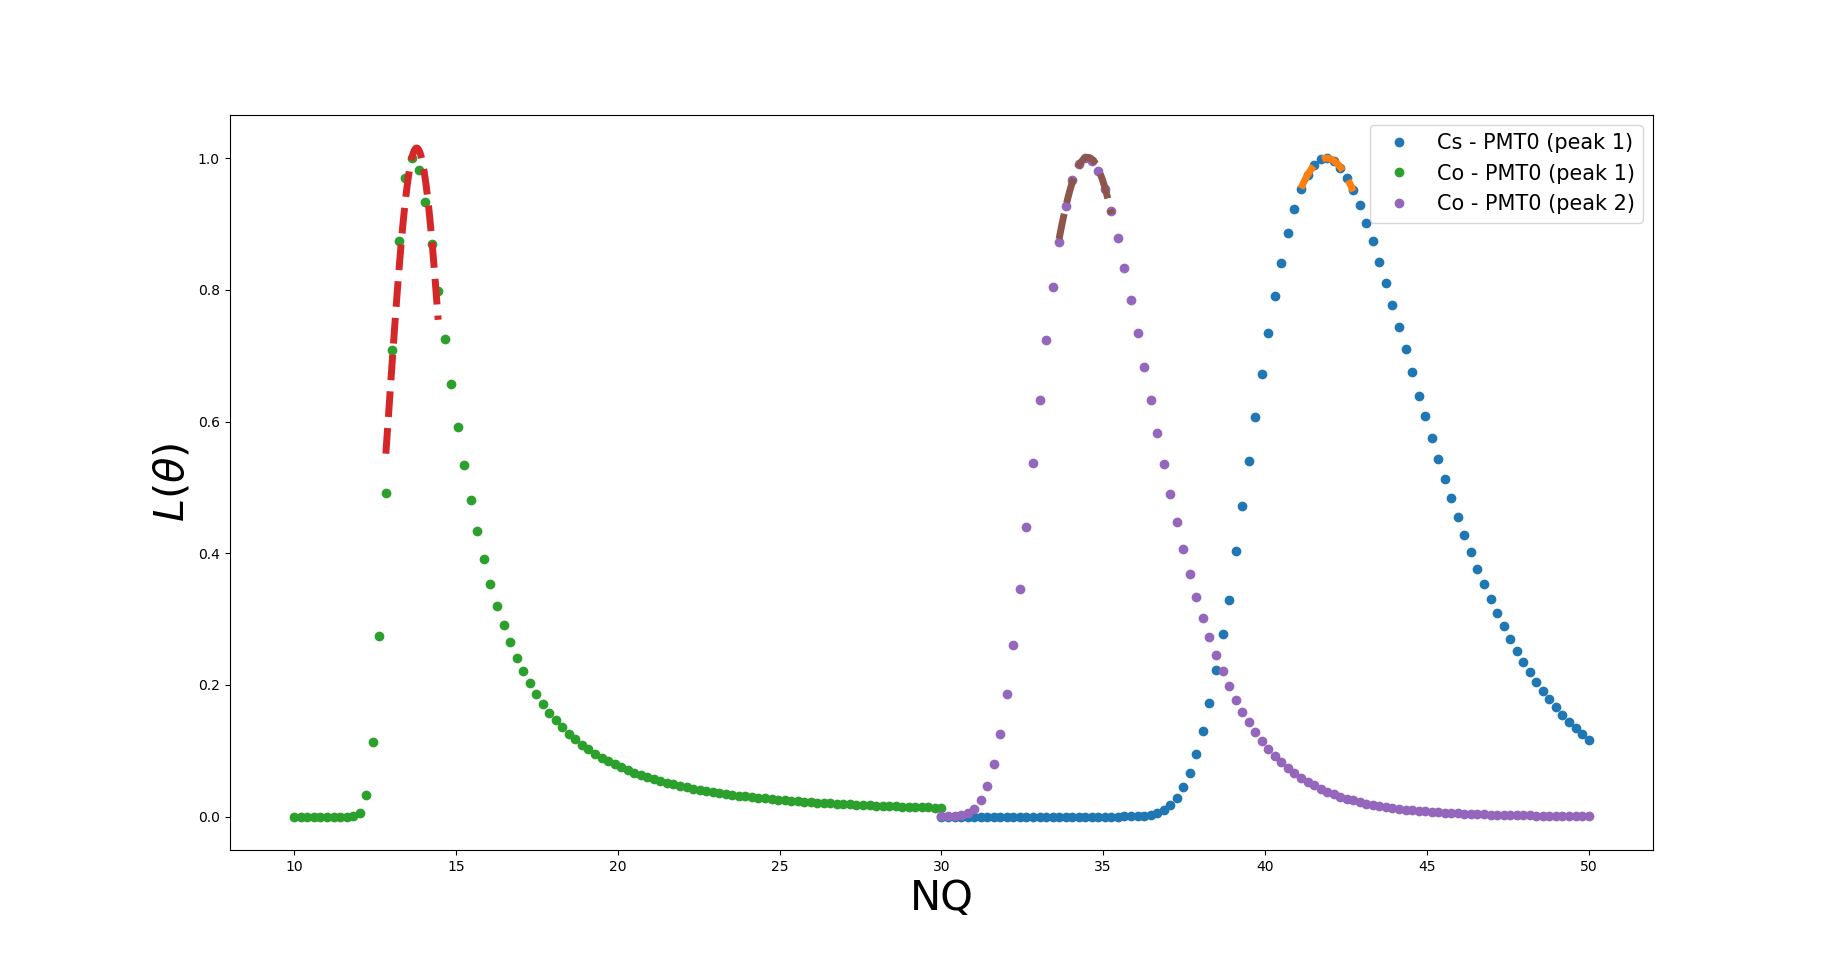
\includegraphics[width=1\linewidth]{NQ.png}
\end{figure}

\begin{center}
\begin{tabular}{ |c| c| c|}
\hline
 Source & $\hat{NQ}$ & $\sigma_{NQ}$\\ 
\hline
Cs & 42 & 2.5\\  
\hline  
Co (peak 1) & 14 & 0.8\\  
\hline  
Co (peak 2) & 34 & 1.7\\ 
\hline
\end{tabular}
\end{center}
\end{frame}


\begin{frame}{F}
\begin{figure}[h]
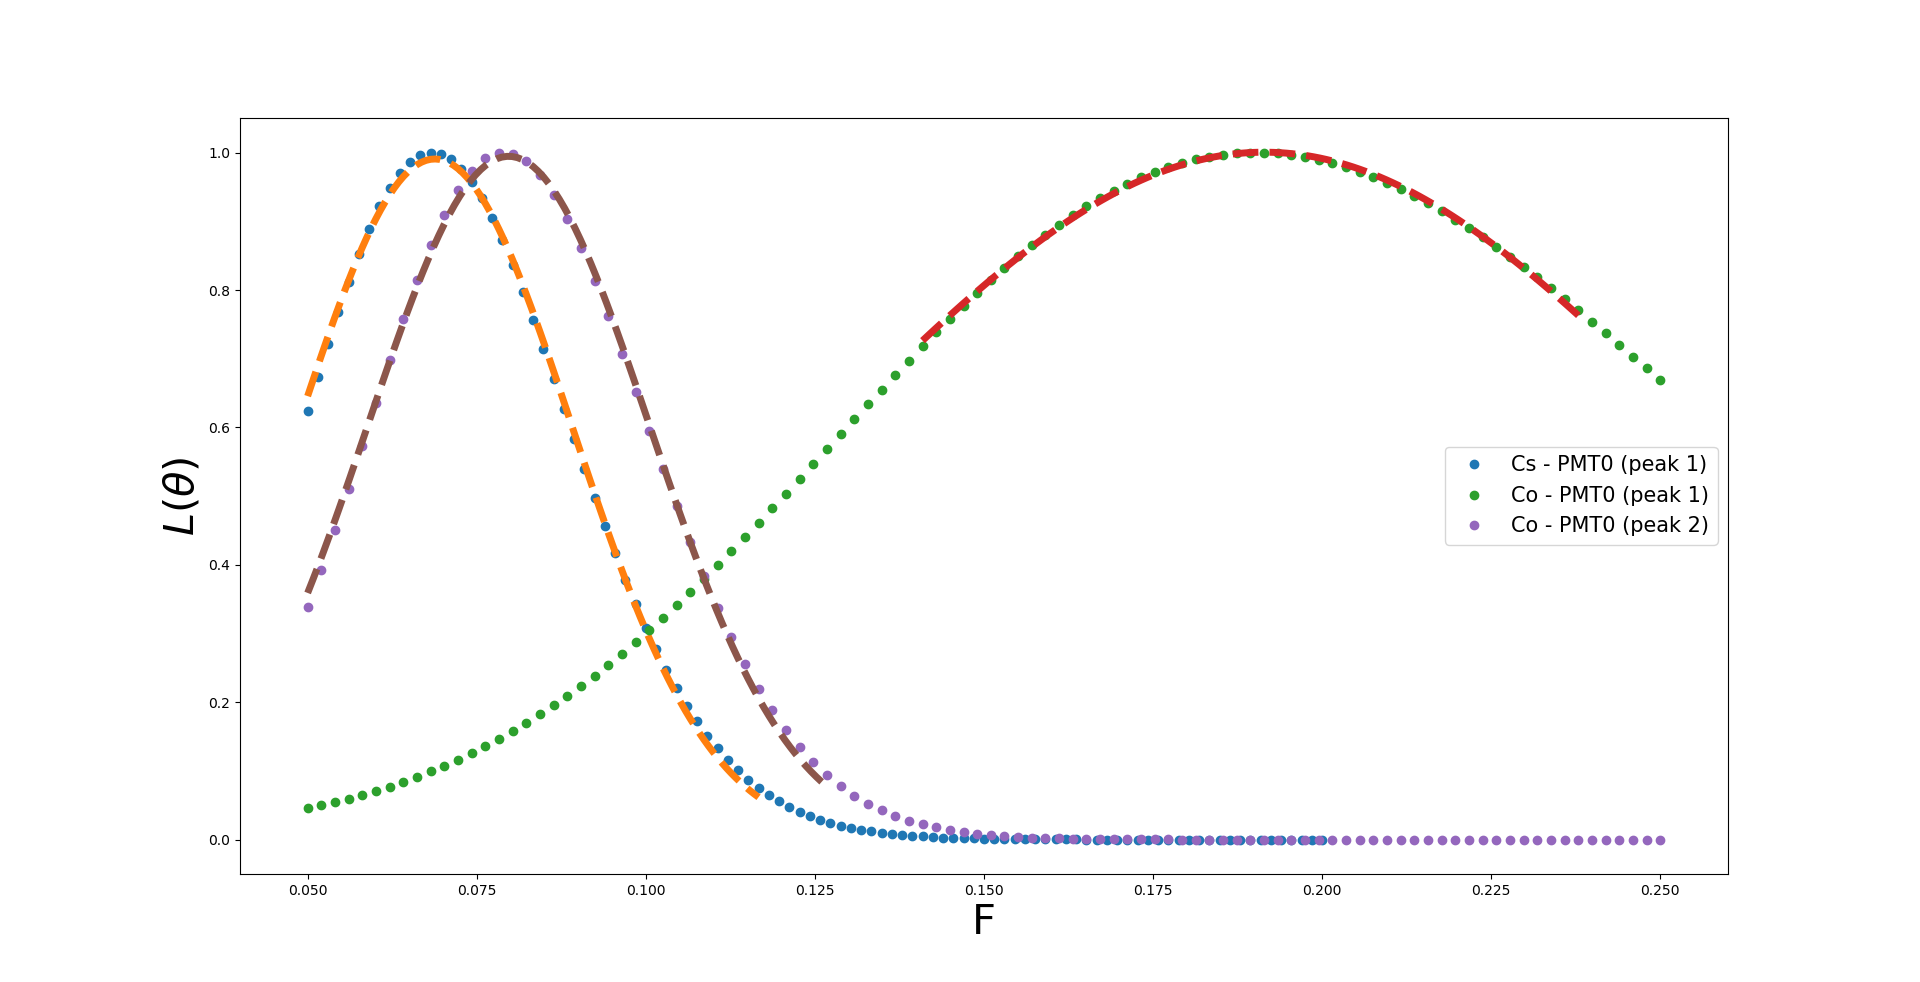
\includegraphics[width=1\linewidth]{F.png}
\end{figure}

\begin{center}
\begin{tabular}{ |c| c| c|c|}
\hline
 Source & $\hat{F}$ & $\sigma_{F}$ & significance [$\sigma$]\\ 
\hline
Cs & 0.07 & 0.02 & 3\\  
\hline  
Co (peak 1) & 0.2 & 0.06 & 3\\  
\hline  
Co (peak 2) & 0.08 & 0.02 & 4\\ 
\hline
\end{tabular}
\end{center}
\end{frame}

\begin{frame}{$\tau_s$}
\begin{figure}[h]
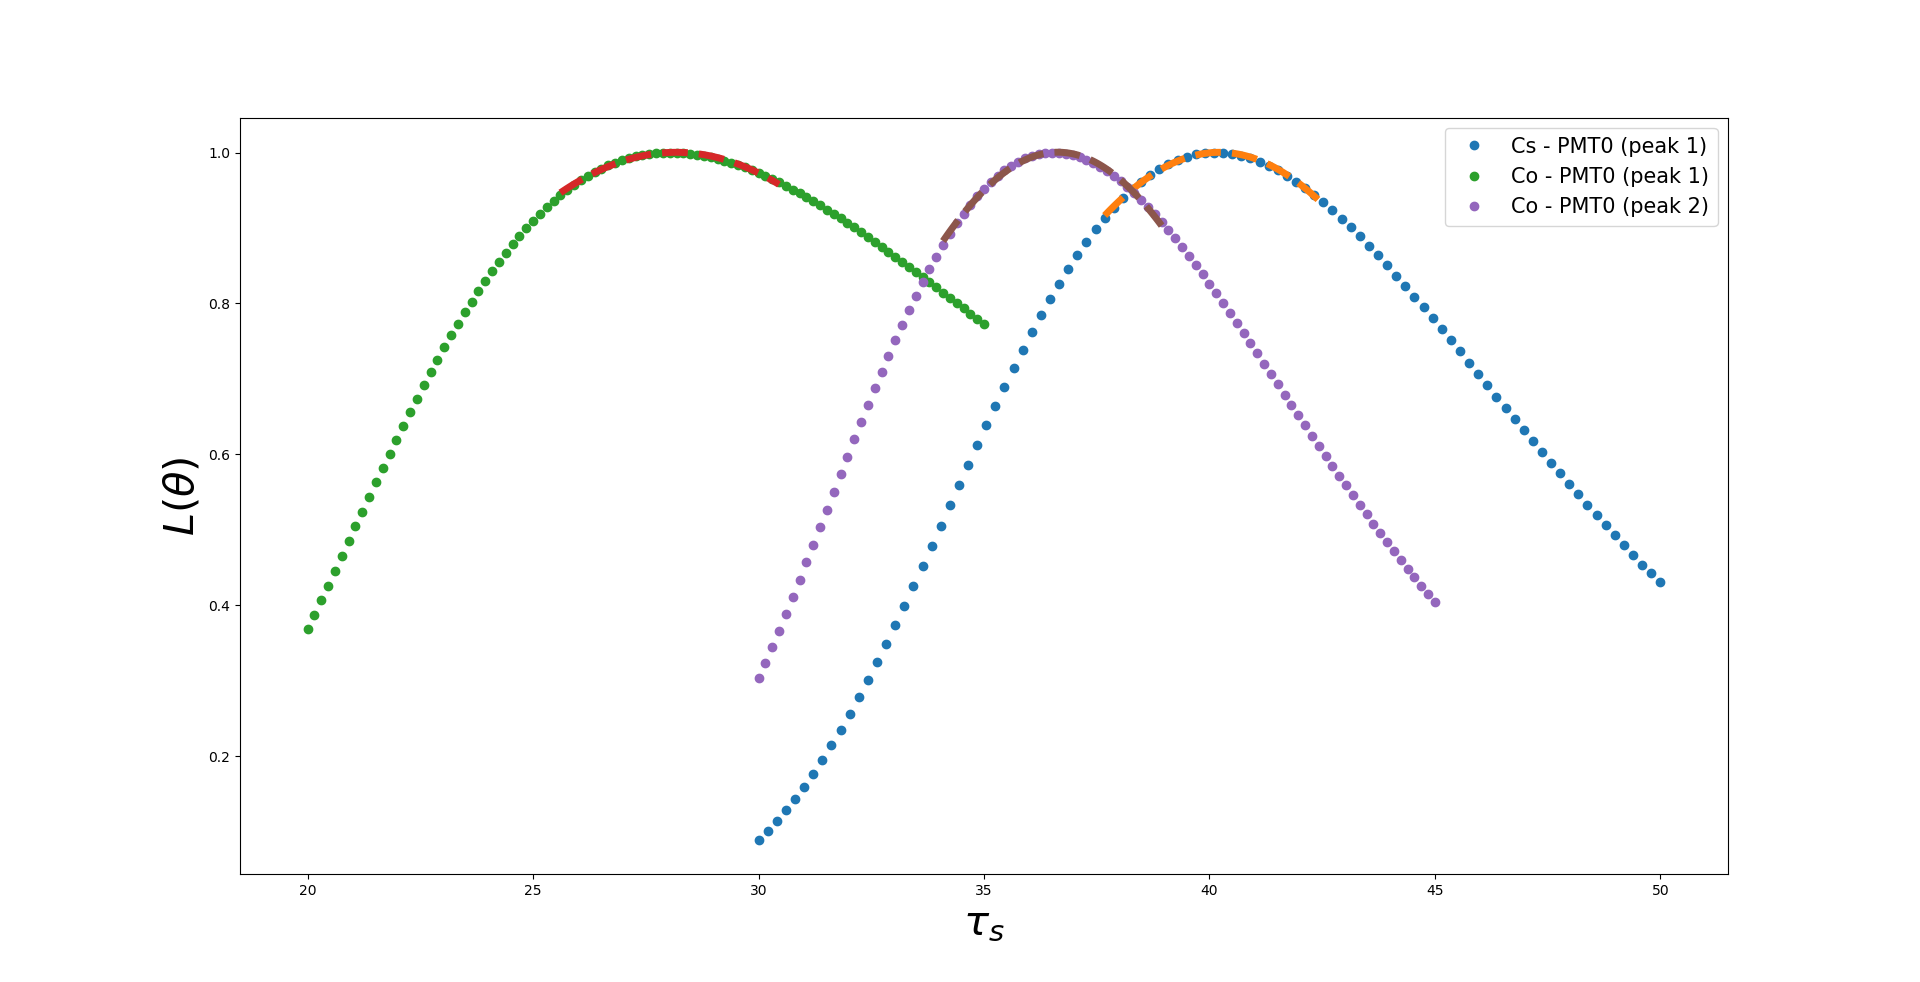
\includegraphics[width=1\linewidth]{Ts.png}
\end{figure}

\begin{center}
\begin{tabular}{ |c| c| c|}
\hline
 Source & $\hat{\tau_s} [ns]$ & $\sigma_{\tau_s} [ns]$\\ 
\hline
Cs & 40 & 6\\  
\hline  
Co (peak 1) & 28 & 8\\  
\hline  
Co (peak 2) & 37 & 5\\ 
\hline
\end{tabular}
\end{center}
\end{frame}

\begin{frame}{How to go on}
\begin{itemize}
\item Preform this analysis for all PMTs individually for both sources and both orientations (source to the lab / to the door).
\item Study the low energy component in the Co spectrum and if it has a different scintillation regime (NR?).
\item Maximize $L$ with the constrain that $N, F, \tau_s $ is the same for all PMTs (but different between sources). This will brake the degeneracy of $NQ$.
\item Maximize $L$ with only $N, \tau_s$ fixed for all PMTs. This will show the anisotropy in the fast component.
\item Maximize $L$ with $N, \tau_s$ fixed and constrain a $90\deg$ between the symmetry axis of the anisotropy of $F$ in the two orientations.
\item Maximize $L$ with the above with the constrain that $F$ is isotropic in the BG data. 
\end{itemize}
\end{frame}
\end{document}

